\chapter{Network and Host Alert Correlation}
\label{correlation}
Either as part of an \ac{IDS} or as a post-processing step, the alert
correlation task is meant to recognize relations among alerts. For
instance, a simple correlation task is to suppress all the alerts
regarding unsuccessful attacks. A more complex example envisions a
large enterprise network monitored by multiple \acp{IDS}, both
host\hyp{} and network\hyp{}based. Whenever a misbehaving application
is detected on a certain machine, the \ac{HIDS} interacts with the
\ac{NIDS} that is monitoring the network segment of that machine to,
say, validate the actual detection result. A more formal definition of
alert correlation and alert correlation systems can be found in
Section~\ref{detection:id:alert-correlation}.

In this section we focus on practical aspects of alert correlation by
first presenting the model we used in our prototype tools. Based on
this model we concentrate on two challenging phases, namely
\emph{aggregation}, which has to do with grouping similar alerts
together, and \emph{correlation}, which is the actual correlation
phase. In particular, in Section~\ref{correlation:fusion} we
investigate the use of fuzzy metrics to time-based aggregation, which
has been proposed recently as a simple but effective aggregation
criterion. Unfortunately, given a threshold of, say, $10s$, this
approach will fail if two alerts are at, say, $10.09s$ to each
other. In Section~\ref{correlation:causality} we focus on the actual
correlation task. We exploit non\hyp{}parametric statistical tests to
create a simple but robust correlation system that is capable of
recognizing series of related events without relying on previous
knowledge. Last, in Section~\ref{correlation:evaluation} we propose a
methodology to compare alert correlation systems which are as
difficult as \acp{IDS} to evaluate.

\section{Fuzzy Models and Measures for Alert Fusion}
\label{correlation:fusion}
In this section we focus on the aggregation of \ac{IDS}\index{IDS}
alerts, an important component of the alert correlation process as
shown on Figure~\ref{fig:correlation_model}. We describe our approach
\citep{2009_maggi_zanero_matteucci_fusion}, which exploit fuzzy
measures and fuzzy sets to design simple and robust alert aggregation
algorithms. Exploiting fuzzy sets, we are able to robustly state
whether or not two alerts are ``close in time'', dealing with noisy
and delayed detections. A performance metric for the evaluation of
fusion systems is also proposed. Finally, we evaluate the fusion
method with alert streams from anomaly-based \ac{IDS}\index{IDS}.

\begin{figure}[t]
  \centering
  \begin{tikzpicture}[node distance=7.5em,every node/.style={inner sep=.5em,font=\footnotesize}]
    \node [draw,shape=rectangle,double copy shadow,fill=white] (ids) {IDS};
    \node (A) [right of=ids,text width=1.2em] {$\mathbb{A}_{1}$\\...\\$\mathbb{A}_{n}$};
    \node [draw,shape=rectangle] (N) [right of=A] {Normalization};
    \node [draw,shape=rectangle] (P) [right of=N] {Prioritization};
    \node [draw,shape=rectangle] (Ag) [below of=P] {Aggregation};
    \node [draw,shape=rectangle] (C) [left of=Ag] {Correlation};
    \node [draw,shape=rectangle] (V) [left of=C] {Verification};
    \node (As) [left of=V] {$\mathbb{A}'$};
    
    \draw[-stealth] (ids) -- (A);
    \draw[-stealth] (A) -- (N);
    \draw[-stealth] (N) -- (P);
    \draw[-stealth] (P) -- (Ag);
    \draw[-stealth] (Ag) -- (C);
    \draw[-stealth] (C) -- (V);
    \draw[-stealth] (V) -- (As);
  \end{tikzpicture}
  \caption{Simplified version of the correlation approach proposed
    in~\citep{valeur04comprehensive}.}
  \label{fig:correlation_model}
\end{figure}

Alert aggregation becomes more complex when taking into account
\emph{anomaly detection} systems, because no information on the type
or classification of the observed attack is available to any of the
fusion algorithms. Most of the algorithms proposed in the current
literature on correlation make use of the information regarding the
matching attack provided by misuse detectors; therefore, such methods
are inapplicable to purely anomaly based intrusion detection
systems. Although some approaches, e.g.,~\citep{1224380}, incorporate
techniques to correlate automatically-generated signatures, such
techniques are aimed at creating more general signatures in order to
augment the DR. Instead, our focus is that of reducing the FPR by
fusing more information sources. However, as described in
Section~\ref{detection:id}, since anomaly and misuse detection are
symmetric, it is reasonable and noteworthy to try to integrate
different approaches through an alert fusion process.

Toward such goal, we explore the use of fuzzy measures
\citep{fuzzymeasure} and fuzzy sets \citep{folger_klir} to design
simple, but robust aggregation algorithms. In particular, we
contribute to one of the key issues, that is how to state whether or
not two alerts are ``close in time''. In addition, uncertainties on
both timestamp measurements and threshold setting make this process
even more difficult; the use of fuzzy sets allows us to precisely
define a time-distance criterion which ``embeds'' unavoidable errors
(e.g., delayed detections).

\subsection{Time-based alert correlation}
\label{correlation:fusion:time-based-alert}
As proposed in most of the reviewed literature, a first, naive
approach consists in exploiting the \emph{time distance} between
alerts for aggregation; the idea is to aggregate ``near'' alerts. In
this section we focus on this point, starting by the definition of
``near''.

Time-distance aggregation might be able to catch simple scenarios like
remote attacks against remote applications vulnerabilities (e.g., web
servers ). For instance, consider the scenario where, at time $t_{0}$,
an attacker violates a host by exploiting a vulnerability of a server
application. An \ac{IDS}\index{IDS} monitoring the system recognizes
anomalous activity at time $t_{n} = t_{0} + \tau_{n}$. Meanwhile, the
attacker might escalate privileges and break through another
application; the \ac{IDS}\index{IDS} would detects another anomaly at
$t_{h} = t_{0} + \tau_{h}$. In the most general case $t_{n}$ is
``close'' to $t_{h}$ (with $t_{n} < t_{h}$), so if $t_{h} - t_{n} \leq
T_{near}$ the two alerts belong to the same attack.

\begin{figure}[p]
  \centering
  
  \subfloat[][]{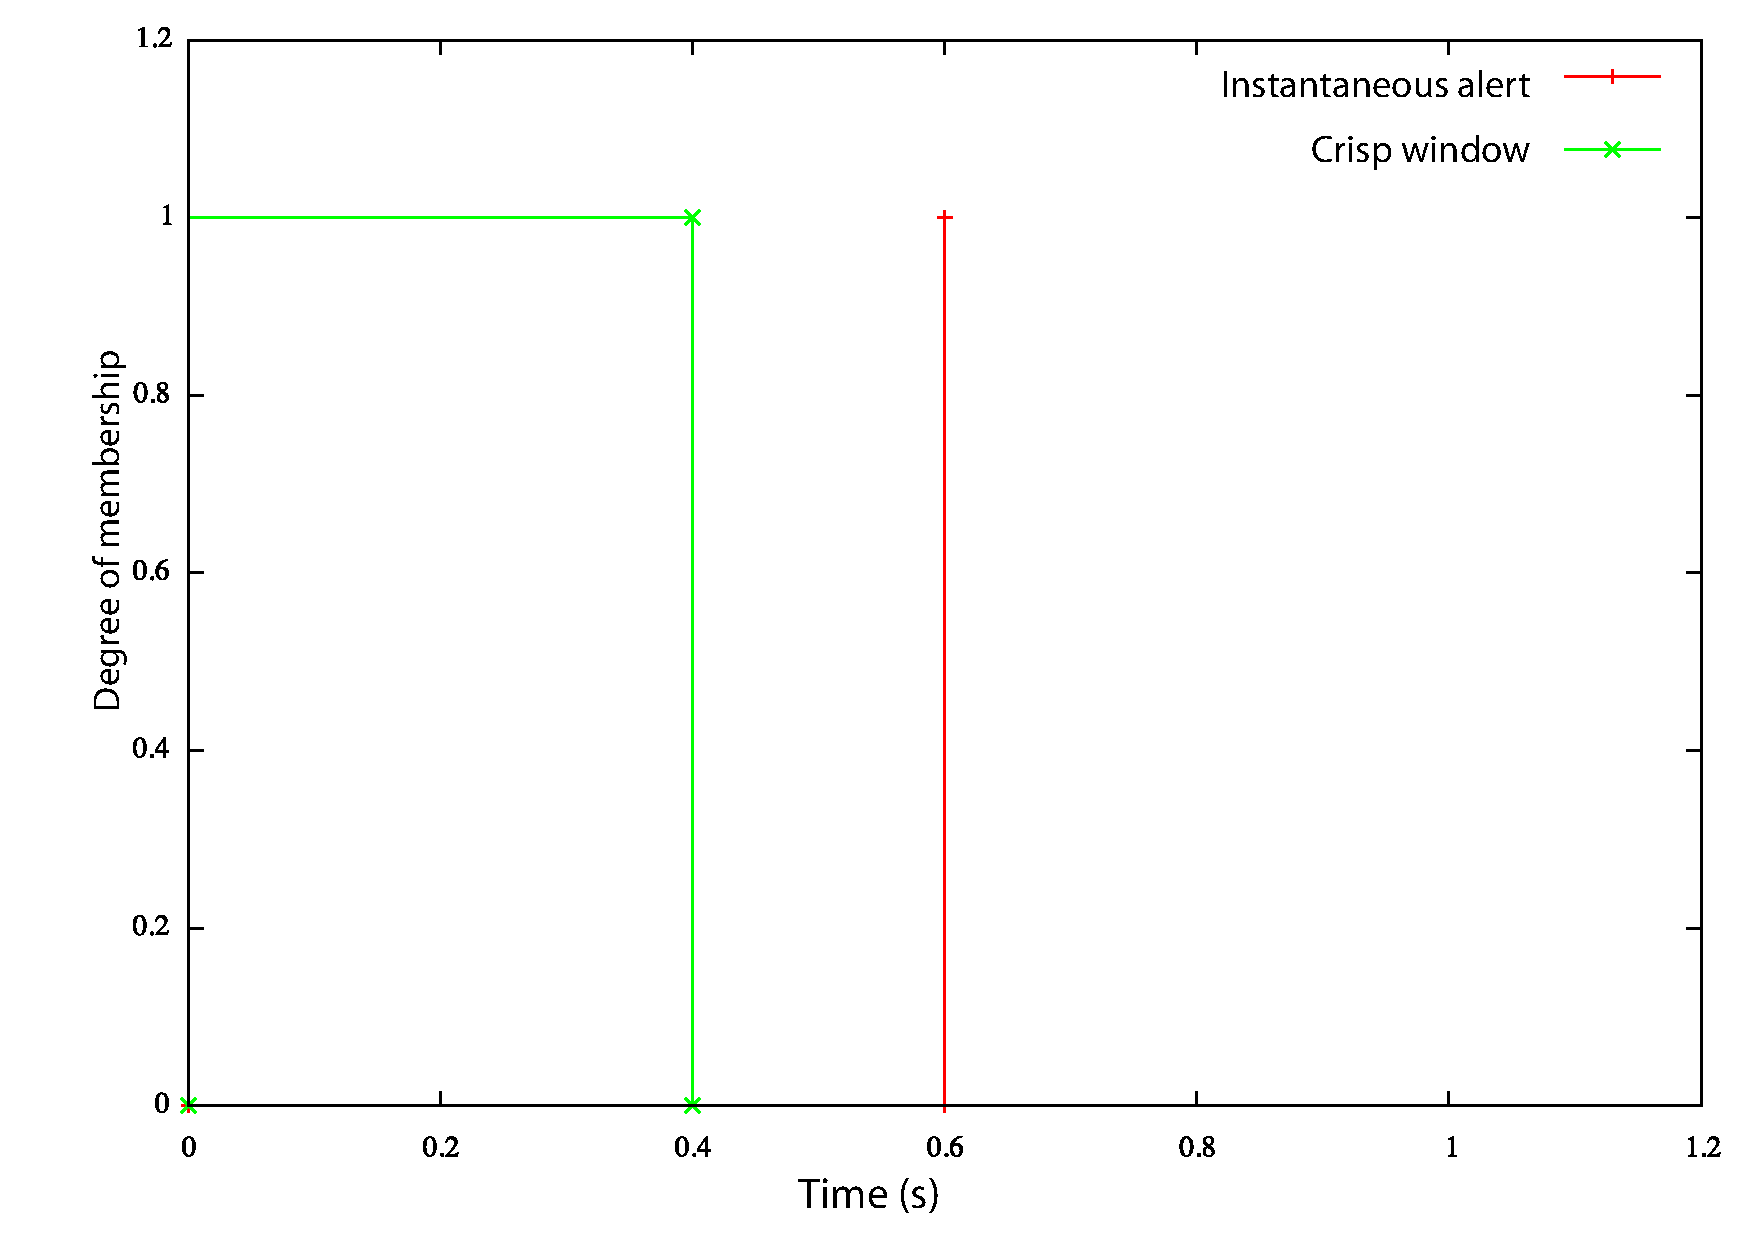
\includegraphics[width=.8\textwidth]{figures/correlation/fusion/fuzzy_crisp_distance}}

  \subfloat[][]{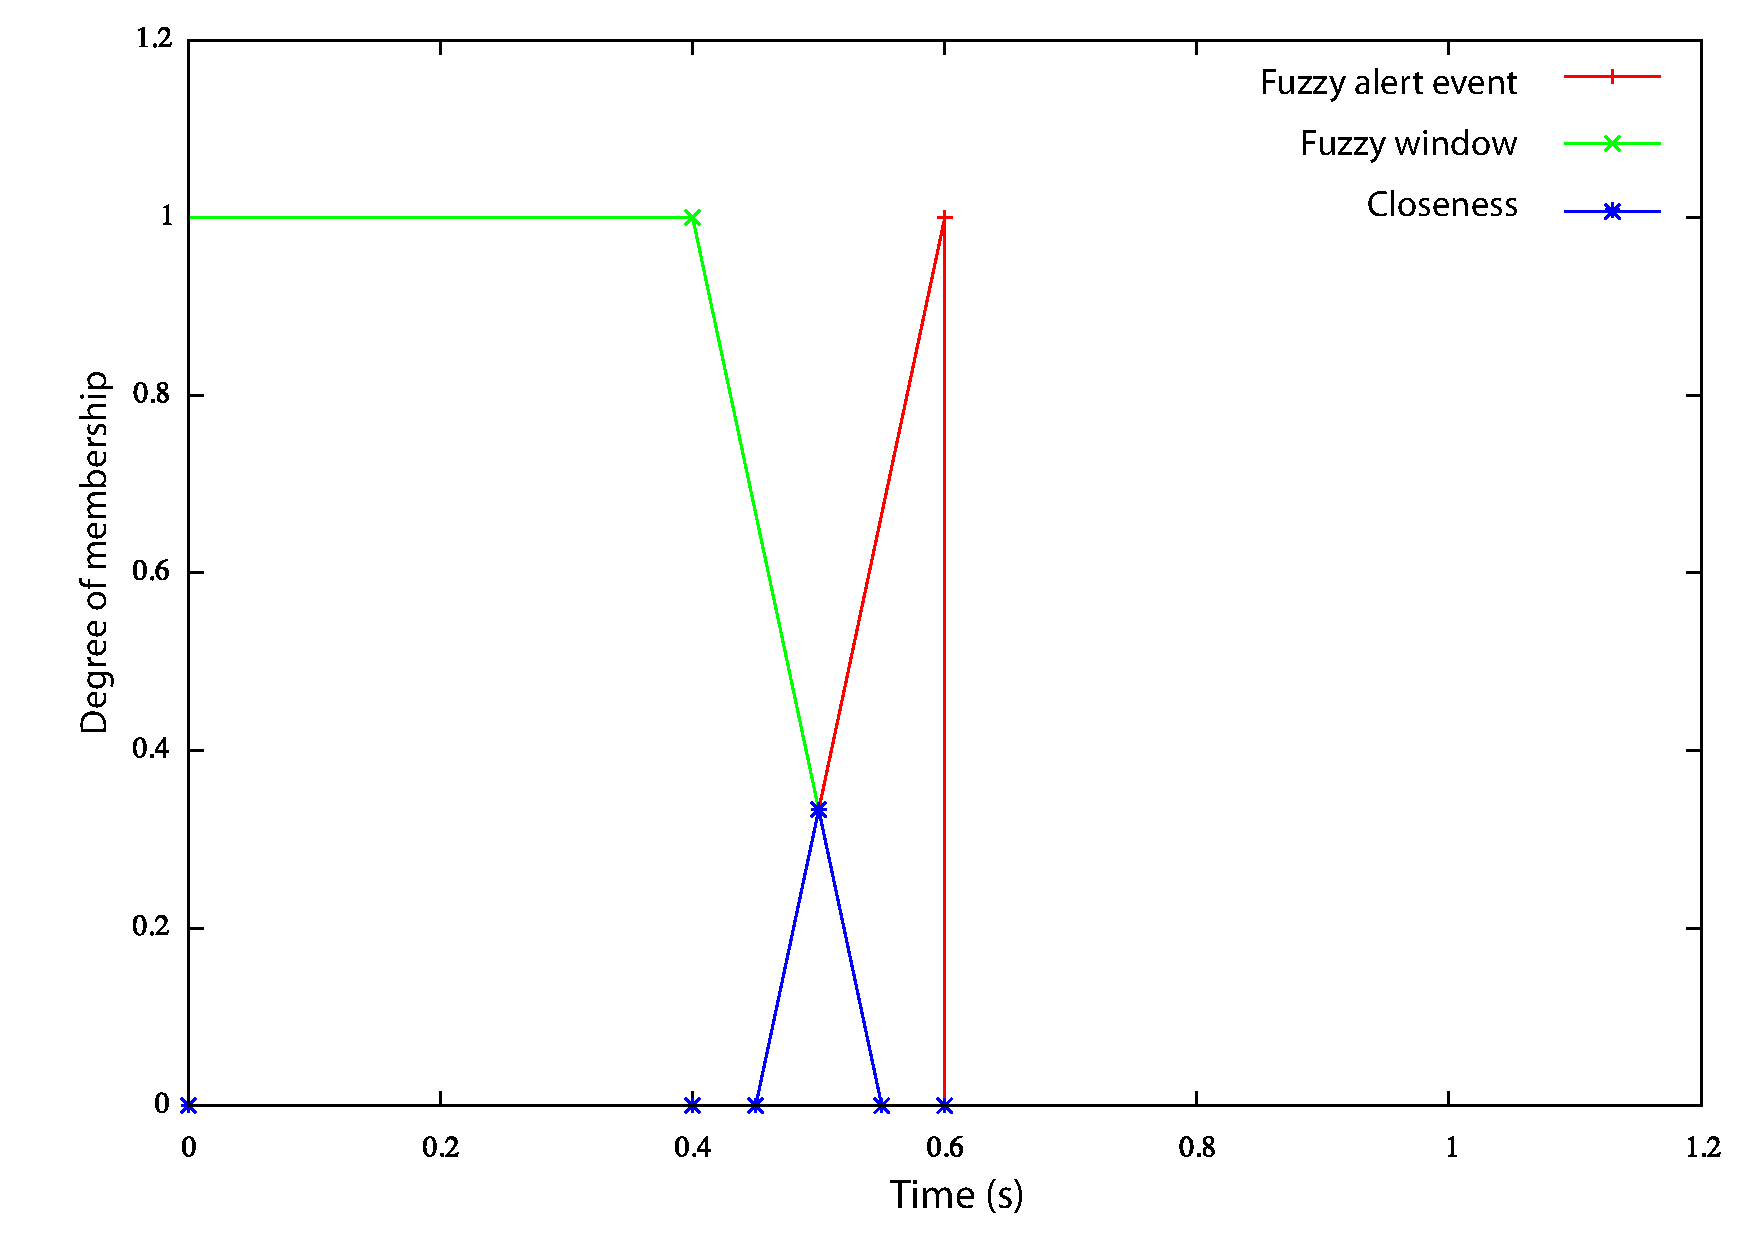
\includegraphics[width=.8\textwidth]{figures/correlation/fusion/fuzzy_distance}}
  
  \caption{Comparison of crisp (a) and fuzzy (b) time-windows. In both
    graphs, one alert is fired at $t = 0$ and another alert occurs at
    $t = 0.6$. Using a crisp time-window and instantaneous alerts (a),
    the distance measurement is not robust to neither delays nor
    erroneous settings of the time-window size. Using fuzzy-shaped
    functions (b) provides more robustness and allows to capture the
    concept of ``closeness'', as implemented with the \textsf{T}-norm
    depicted in (b). Distances in time are normalized in [0,1]
    (w.r.t. the origin).}
  \label{fig:crisp_fuzzy_distance}
\end{figure}

The idea is to \emph{fuse} alerts if they are both close in time, raised from the same \ac{IDS}\index{IDS}, and refer to the same source and destination. This intuition obviously needs to be detailed. First, the concept of ``near'' is not precisely defined; secondly, errors in timestamping are not taken into account; and, a crisp time distance measure is not robust. For instance, if $|t_{h} - t_{n}| = 2.451$ and $T_{near} = 2.450$ the two alerts are obviously near, but not aggregated, because the above condition is not satisfied. To overcome such limitations, we propose a \emph{fuzzy} approach to time-based aggregation.

In the following, we will use the well-known dot notation, as in object-oriented programming languages, to access a specific alert attribute: e.g., $a.start\_ts$ indicates the value of the attribute $start\_ts$ of the alert $a$. Moreover, we will use $T_{(\cdot)}$ to indicate a threshold variable: for instance, $T_{near}$ is the threshold variable called (or regarding to) ``near''.

We rely on fuzzy sets for modeling both the uncertainty on the timestamps of alerts and the time distance in a robust manner. Regarding the uncertainty on measurements, we focus on delayed detections by using triangle-shaped fuzzy sets to model the occurrence of an alert. Since the measured timestamp may be affected by errors or delays, we extend the singleton shown in Figure \ref{fig:crisp_fuzzy_distance} (a) with a triangle, as depicted in Figure \ref{fig:crisp_fuzzy_distance} (b). We also take into account uncertainty on the dimension of the aggregation window: instead of using a crisp window (as in Figure \ref{fig:crisp_fuzzy_distance} (a)), we extend it to a trapezoidal fuzzy set, resulting in a more robust distance measurement. In both graphs, one alert is fired at $t = 0$ and another alert occurs at $t = 0.6$. Using a crisp time-window and instantaneous alerts (Figure \ref{fig:crisp_fuzzy_distance} (a)), the distance measurement is not robust to neither delays nor erroneous settings of the time-window size. Using fuzzy-shaped functions (Figure \ref{fig:crisp_fuzzy_distance} (b)) provides more robustness and allows to capture the concept of ``closeness'', as implemented with the \textsf{T}-norm depicted in Figure \ref{fig:crisp_fuzzy_distance} (b). In Figure \ref{fig:crisp_fuzzy_distance} distances in time are normalized in [0,1] (w.r.t. the origin).

Note that, Figure \ref{fig:fuzzy_delay} compares two possible manners to model uncertainty on alert timestamps: in Figure \ref{fig:fuzzy_delay} (a) the alert is recorded at 0.5 seconds but the measurement may have both positive (in the future) and negative (in the past) errors. Figure \ref{fig:fuzzy_delay} (b) is more realistic because positive errors are not likely to happen (i.e., we cannot ``anticipate'' detections), while events are often delayed, especially in network environments. In comparison to our proposal of using ``fuzzy timestamps'', the \ac{IDMEF} describes event occurrences using \emph{three} timestamps (\texttt{Create-}, \texttt{Detect-}, and \texttt{Analyzer-Time}): this is obviously more generic and allows the reconstruction of the entire event path from the attack to the analyzer that reports the alert. However, all timestamps are not always known: for example, the \ac{IDS} might not have such a feature, thus the \ac{IDMEF} \texttt{Alert}s cannot be completely filled.

\begin{figure}[p]
  \centering
  \subfloat[][]{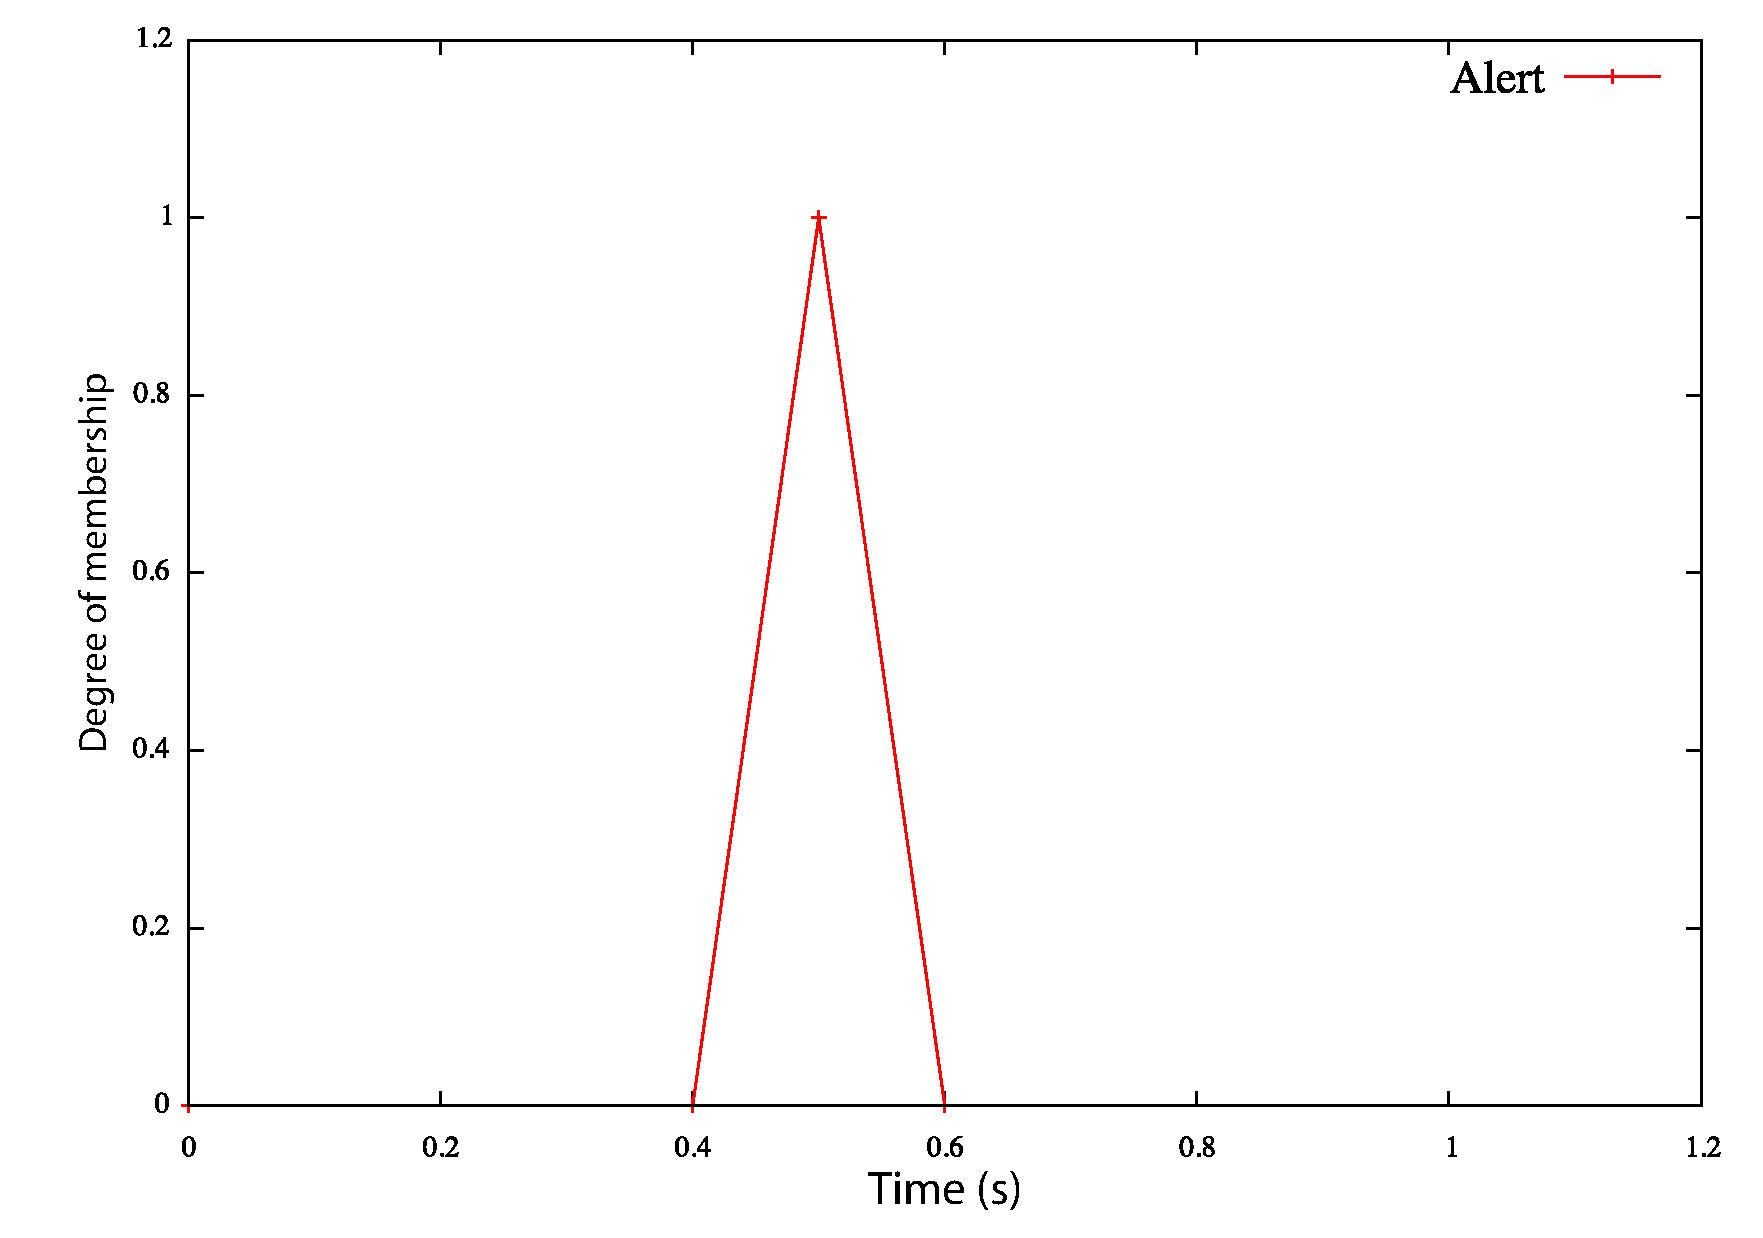
\includegraphics[width=0.8\textwidth]{figures/correlation/fusion/fuzzy_alert_delay}
  }\\

  \subfloat[][]{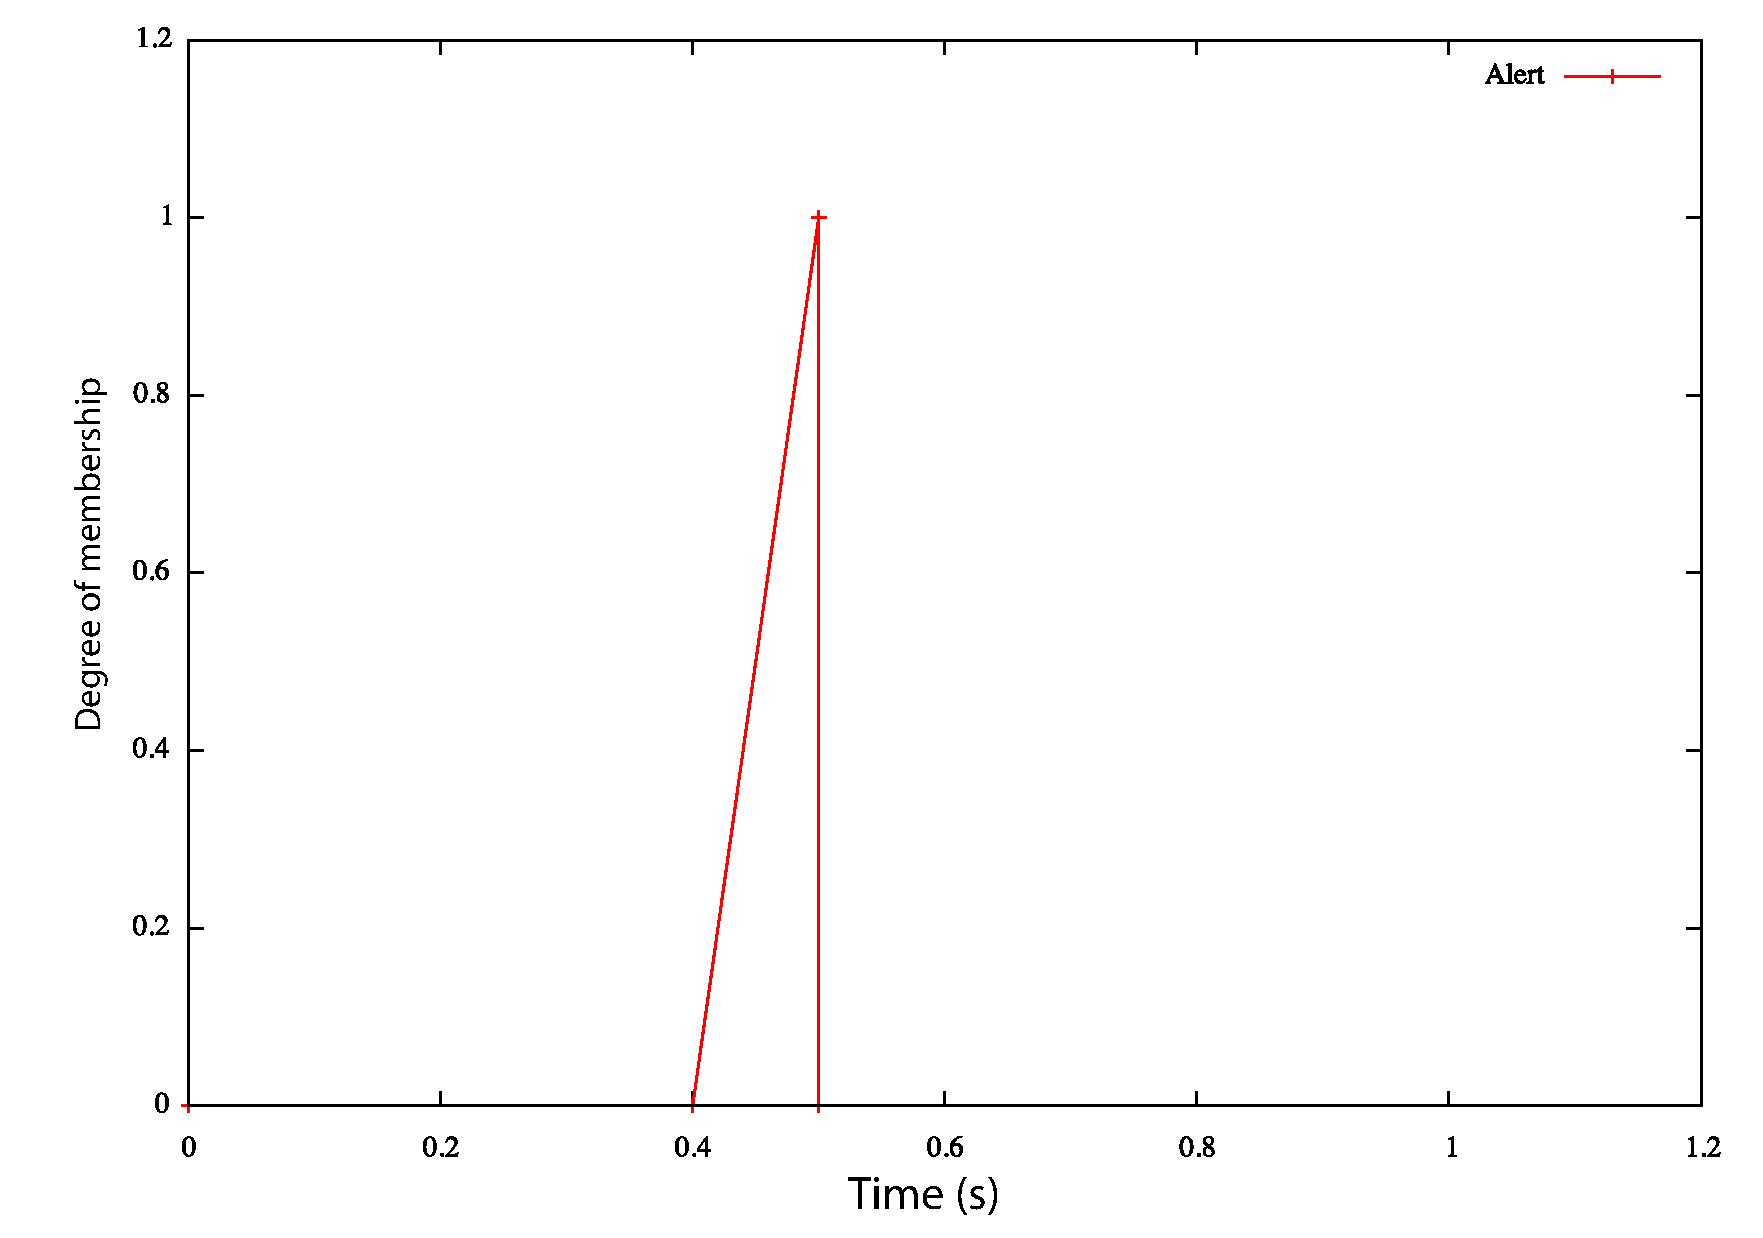
\includegraphics[width=0.8\textwidth]{figures/correlation/fusion/fuzzy_alert_delay_ok}}
  
  \caption{Comparing two possible models of uncertainty on timestamps of single alerts.}
  \label{fig:fuzzy_delay}
\end{figure}

As stated above, the main goal is to measure the time distance between two alerts, $a_{1}$ and $a_{2}$ (note that, in the following, $a_{2}$ occurs after $a_{1}$). We first exemplify the case of instantaneous alerts, that is $a_{i}.start\_ts = a_{i}.end\_ts = a_{i}.ts$ for $i \in \{1, 2\}$. To state whether or not $a_{1}$ is close to $a_{2}$ we use a $T_{near}$ sized time window: in other words, an interval spreading from $a_{1}.ts$ to $a_{1}.ts + T_{near}$ (Figure \ref{fig:crisp_fuzzy_distance} (a) shows the described situation for $a_{1}.ts = 0$, $T_{near} = 0.4$, and $a_{2}.ts = 0.6$: values have been normalized to place $a_{1}$ alert in the origin).

Extending the example shown in Figure \ref{fig:crisp_fuzzy_distance} (a) to uncertainty in measurements is straightforward; let us suppose to have an average uncertainty of 0.15 seconds on the measured (normalized w.r.t. the origin) value of $a_{2}.ts$: we model is as a triangle-shaped fuzzy set as the one drawn in Figure \ref{fig:crisp_fuzzy_distance} (b).

In the second place, our method takes into account uncertainty regarding the thresholding of the distance between two events, modeled in Figure \ref{fig:crisp_fuzzy_distance} (b) by the trapezoidal fuzzy window: the smoothing factor, 0.15 seconds, represents potential errors (i.e., the time values for which the membership function is neither 1 nor 0). Given these premises, the fuzzy variable ``near'' is defined by a T-norm \citep{folger_klir} as shown in Figure \ref{fig:crisp_fuzzy_distance} (b): the resulting triangle represents the alerts overlapping in time. In the example we used $\mathrm{min}(\cdot)$ as T-norm.

In the above examples, simple triangles and trapezoids have been used
but more accurate/complex membership functions could be used as
well. However, we remark here that trapezoid-like sets are
conceptually different from triangles as the former have a membership
value of 100\%; this means certainty on the observed/measured
phenomenon (i.e., closeness), while lower values mean
uncertainty. Trapezoids-like functions should be used whenever a
100\%-certainty interval is known: for instance, in Figure
\ref{fig:crisp_fuzzy_distance} (b) if two alerts occur within 0.4
seconds they are near at 100\%; between 0.4 and 0.55 seconds, such
certainty decreases accordingly.

\begin{note}[Extended crisp window]
  It is important to underline that, from a purely practical point of
  view, one may achieve the same effect on alert fusion by building a
  more ``flexible'' crisp time window (e.g., by increasing its size
  by, say, 15\%). However, from a theoretical point of view, it must
  be noted that our approach explicitly models the errors that occur
  during the alert generation process. On the other hand, by
  increasing a time window of a certain percentage would only give
  more flexibility, without giving any semantic definition of ``near
  alerts''. There is a profound difference between saying ``15\%
  larger'' and assigning a precise membership function to a certain
  variable and defining T-norms for aggregation.
\end{note}

The approach can be easily generalized to take into account
non\hyp{}instantaneous events, i.e. $a_{i}.start\_ts <
a_{i}.end\_ts$. In this case, alerts delays have to be represented by
a trapezoidal fuzzy set. Note that, smoothing parameters are
configurable values as well as fuzzy set shapes, in order to be as
generic as possible w.r.t. the particular network environment; in the
most general case, such parameters should be estimated before the
system deployment. In Figure \ref{fig:fuzzy_alert_trapez} the measured
value of $a_{i}.start\_ts$ is $0.4$, while $a_{i}.end\_ts = 0.8$;
moreover, a smoothing factor of 0.15 seconds is added as a negative
error, allowing the real $a_{i}.start\_ts$ to be 0.25.

\begin{figure}[t]
  \centering
  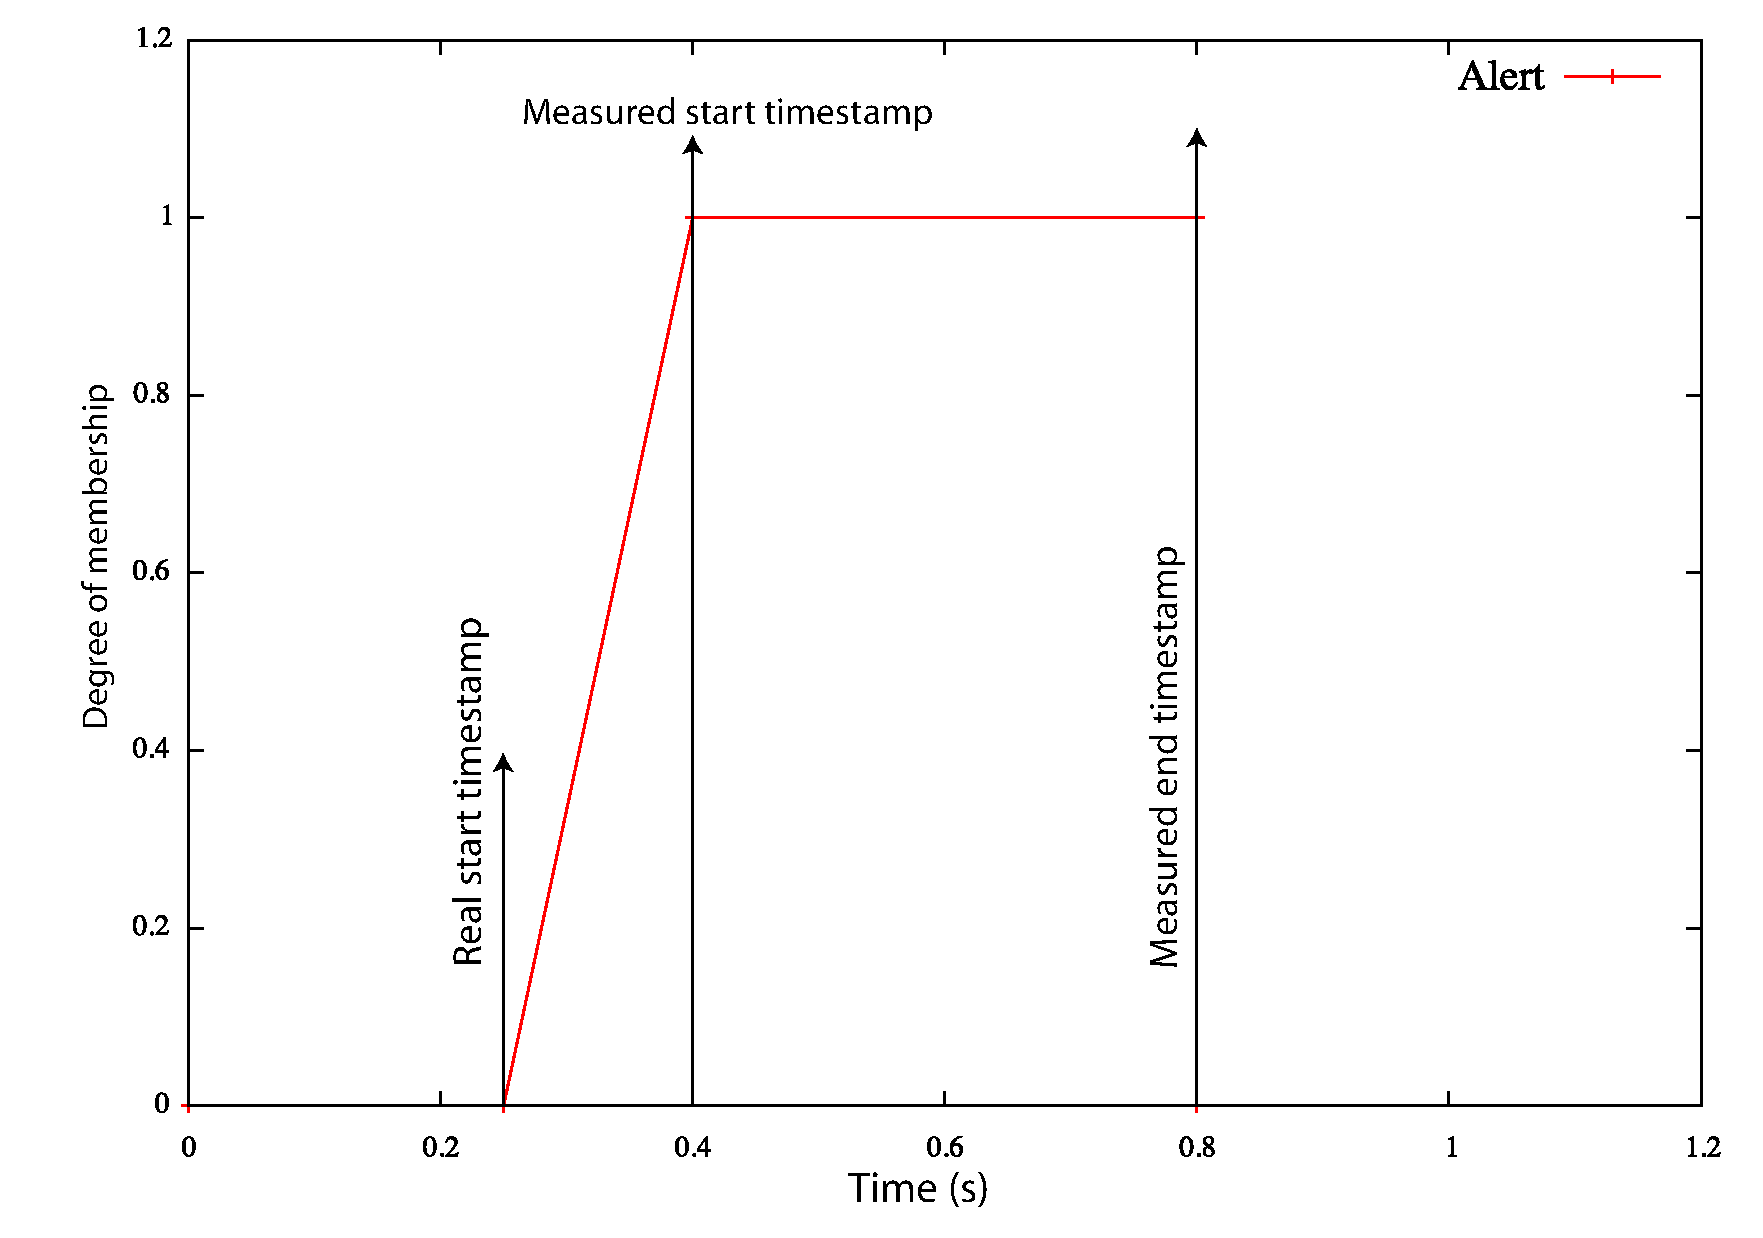
\includegraphics[width=\textwidth]{figures/correlation/fusion/fuzzy_alert_trapez}
  \caption{Non-zero long alert: uncertainty on measured timestamps are modeled.}
  \label{fig:fuzzy_alert_trapez}
\end{figure}

\subsubsection{Alert pruning}
\label{correlation:fusion:fuzzy-based-pruning}
As suggested by the \ac{IDMEF}\index{IDMEF} \texttt{Confidence} attribute both the \ac{IDS} described in Chapter~\ref{host} and \citep{zanero-savaresi,zanero-pattern} --- that we also use in the following experiments --- feature an \texttt{attack\_belief} value. For a generic alert $a$ the \texttt{attack\_belief} represents the deviation of the anomaly score, $a.score$, from the threshold, $T$. The concept of anomaly score is typical of anomaly detectors and, even if there is no agreement about its definition, it can intuitively interpreted as an internal, absolute indicator of abnormality. To complete our approach we consider the \texttt{attack\_belief} attribute for alert pruning, after the aggregation phase.

Many \acp{IDS}\index{IDS}, including the ones that we proposed, rely on probabilistic scores and thresholds in order to isolate anomalies from normal activity; thus, we implemented a first naive belief measure:

\begin{equation}\label{eq:bel}
  \mathrm{Bel}(a) = |a.score - T_{anomaly}| \in [0, 1]
\end{equation}

We remark that $a.score \in [0,1] \wedge T_{anomaly} \in [0,1] \Rightarrow \mathrm{Bel}(a) \in [0, 1]$. Also note that in the belief theory \citep{fuzzymeasure,folger_klir} $\mathrm{Bel}(B)$ indicates the belief associated to the hypothesis (or proposition) $B$; with an abbreviate notation, we indicate $\mathrm{Bel}(a)$ meaning the belief of the proposition ``the alert $a$ is associated to a real anomaly''. In this case, the domain of discourse is the set of all the alerts, which contains both the alerts that are real anomalies and the alerts that are not.

The belief theory has been used to implement complex decision support systems, such as \citep{mycin}, in which a more comprehensive belief model has been formalized taking into account both belief and misbelief. The event (mis)belief basically represents the amount of evidence is available to support the (non-)occurrence of that event. In a similar vein, we exploit both the belief and the \emph{a-priori} misbelief, the \ac{FPR}. The \ac{FPR} tells how much the anomaly detector is likely to report false alerts (i.e., the \emph{a-priori} probability of reporting false alerts, or the so called \emph{type I error}), thus it is a good candidate for modeling the misbelief of the alert. The more the \ac{FPR} increases, the more the belief associated to an alert should decrease. In the first place, such intuition can be formalized using a linear-scaling function:

\begin{equation}\label{eq:bel_lin}
  \mathrm{Bel}_{lin}(a) = (1-\underbrace{FPR}_{\mathrm{misbelief}})\mathrm{Bel}(a)
\end{equation}

However, such a scaling function (see, dashed-line plot in Figure \ref{fig:bel_fpr}) makes the belief to decrease too fast w.r.t. the misbelief. As Figure \ref{fig:bel_fpr} shows, a smoother rescaling function is the following:

\begin{equation}\label{eq:bel_exp}
  \mathrm{Bel}_{exp}(a) = (1-FPR) \mathrm{Bel}(a) e^{FPR}
\end{equation}

\begin{figure}[t]
  \centering
  
  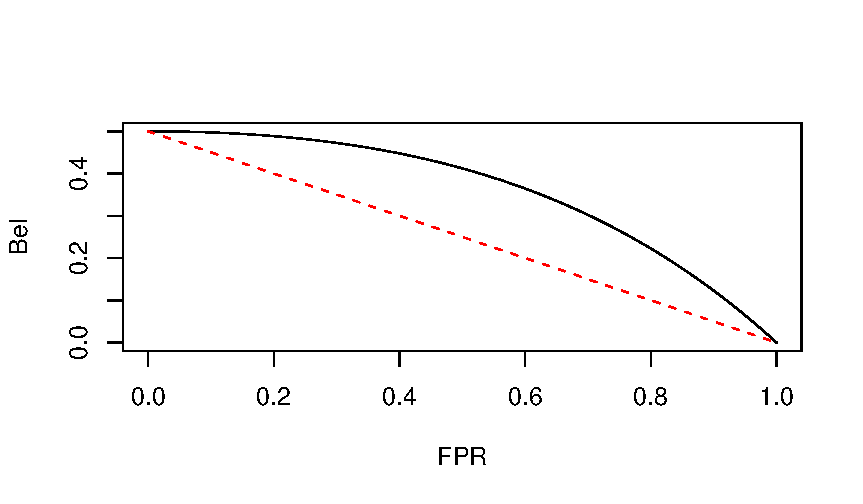
\includegraphics[width=0.8\textwidth]{figures/correlation/fusion/bel_fpr}
  
  \caption{A sample plot of $\mathrm{Bel}_{exp}(a)$ (with $|a.score -
    T_{anomaly}|, FPR \in [0,1]$) compared to a linear scaling
    function, i.e. $\mathrm{Bel}_{lin}(a)$ (dashed line)}
  \label{fig:bel_fpr}
\end{figure}

The above defined \texttt{attack\_belief} is exploited to further
reduce the resulting set of alerts. Alerts are reported only if

\begin{displaymath}
  a_{i}.attack\_belief > T_{bel}
\end{displaymath}

\noindent where $T_{bel}$ must be set to reasonable values according
to the particular environment (in our experiments we used 0.66). The
attack belief variable may be modeled using fuzzy variables with, for
example, three membership functions labeled as ``Low'', ``Medium'',
and ``High'' (\ac{IDMEF}\index{IDMEF} uses the same three-values
assignment for each alert \texttt{Confidence} attribute and we used
crisp numbers for it), but this has not been implemented yet in our
working prototype.

Let us now to summarize the incremental approaches; the first
``\emph{naive time-distance}'' uses a crisp window (as in Figure
\ref{fig:crisp_fuzzy_distance} (a)) to groups alerts w.r.t. their
timestamps. The second approach, called ``\emph{fuzzy
  time-distance}'', extends the first method: it relies on fuzzy sets
(as shown in Figure \ref{fig:crisp_fuzzy_distance} (b)) to take into
account uncertainty on timestamping and window sizing. The last
version, ``\emph{fuzzy time-distance with belief-based alert
  pruning}'', includes the last explained criterion. In the following
we will show the results of the proposed approaches on a realistic
test bench we have developed using alerts generated by our
\ac{IDS}\index{IDS} on the complete \ac{IDEVAL}\index{IDEVAL} testing
dataset (both host and network data).

\section{Mitigating Evaluation Issues}
\label{correlation:evaluation}
This section investigates the problem of testing an alert fusion engine. In order to better understand the data we used, the experimental setup is here detailed and, before reporting the results obtained with the fuzzy approach introduced, we also briefly sketch the theoretical foundations, the accuracy, and the peculiarities of the overall implementation of the \acp{IDS}\index{IDS} used for gathering the alerts. At the end of the section, we compare the results of the aggregation phase in comparison with an analysis of the accuracy of an alternative fusion approach \citep{dblp:conf/raid/qinl03}.

\subsection{A common alert representation}
\label{correlation:evaluation:representation}
The output format of our prototypes has been designed with \ac{IDMEF}\index{IDMEF} in mind, to make the normalization process --- the first step Figure~\ref{fig:correlation_model} --- as straightforward as possible. Being more precise, alerts are reported by our tools as a modified version of the original \textsf{Snort} \citep{snortsite} alert format, in order to take into account both the peculiarities of the anomaly detection approach, namely the lack of attacks name, and suggestions from the \ac{IDMEF}\index{IDMEF} data model. In this way, our testing tools can easily implement conversion procedures from and to \ac{IDMEF}\index{IDMEF}.

Basically, we represent an alert as a tuple with the following 9 attributes:

\begin{center}\footnotesize\ttfamily
  (ids\_id, src, dst, ids\_type, start\_ts, end\_ts, attack\_class, attack\_bel, target\_resource)
\end{center}

The \texttt{ids\_id} identifies the \ac{IDS}\index{IDS}, of type \texttt{ids\_type} (host or network), that has reported the alert; \texttt{src} and \texttt{dst} are the \ac{IP}\index{IP} source and destination addresses, respectively; \texttt{start\_ts} and \texttt{end\_ts} are the detection \ac{NTP}\index{NTP} \citep{RFC1305} timestamps: they are both mandatory, even if the alert duration is unknown (i.e., \texttt{start\_ts} equals \texttt{end\_ts}). The discrete attribute \texttt{attack\_class} (or name) indicates the name of the attack (if known); anomaly detectors cannot provide such an information because recognized attacks names are not known, by definition. Instead, anomaly detectors are able to quantify ``how anomalous an activity is'' so we exploited this characteristic and defined the \texttt{attack\_belief}. Finally, the \texttt{target\_resource} attribute stores the \ac{TCP}\index{TCP} port (or service name), if known, or the program begin attacked. An example instance is the following one:

\begin{center}\footnotesize\ttfamily
  (127.0.0.1-z7012gf, 127.0.0.1, 127.0.0.1, H, 0xbc723b45.0xef449129, 0xbc723b45.0xff449130, -, 0.141044, fdformat(2351))
\end{center}

The example reports an attack detected from an host \ac{IDS}\index{IDS} (\texttt{ids\_type = H}), identified by \texttt{127.0.0.1-z7012gf}: the attack against \texttt{fdformat} is started at NTP-second 0xbc723b45 (picosecond 0xef449129) and finished at NTP-second 0xbc723b45 (picosecond 0xff449130); the analyzer detected the activity as an attack with a belief of 14.1044\%. An equivalent example for the network \ac{IDS}\index{IDS} (\texttt{ids\_type = N}) anomaly detector would be something like:

\begin{center}\footnotesize\ttfamily
  (172.16.87.101/24-a032j11, 172.16.87.103/24, 172.16.87.100/24, N, 0xbc723b45.0xef449129, 0xbc723b45.0xff449130, -, 0.290937, smtp)
\end{center}

Here the attack is against the \texttt{smtp} resource (i.e., protocol) and the analyzer believes there is an attack at 29.0937\%.

\subsection{Proposed Evaluation Metrics}
\label{correlation:evaluation:framework}
Alert fusion is a relatively new problem, thus evaluation techniques are limited to a few approaches \citep{correlation_evaluation}. The development of solid testing methodologies is needed from both the theoretical and the practical points of view (a problem shared with \ac{IDS}\index{IDS} testing).

The main goal of fusion systems is to reduce the amount of alerts the security analyst has to check. In doing this, the \emph{global} \ac{DR} should ideally not decrease while the \emph{global} \ac{FPR} should be reduced as much as possible. This suggests that the first sub-goal of fusion systems is the \emph{reduction} of the \emph{global} \ac{FPR} (for instance, by reducing the total number of alerts fired by source \ac{IDS}\index{IDS} through a rejection mechanism). Moreover, the second sub-goal is to limit the decreasing of the \emph{global} \ac{DR}\index{DR}. Let us now formalize the concepts we just introduced.

We indicate with $\mathbb{A}_{i}$ the \emph{alert set} fired by the $i$-th \ac{IDS}\index{IDS}. An \emph{alert stream} is actually a structure $\langle\mathbb{A}_{i}, \prec\rangle$ over $\mathbb{A}_{i}$, where the binary relation $\prec$ means ``occurs before''. More formally

\begin{eqnarray*}
 &&\forall a, a' \in \mathbb{A}_{i}: a \prec a' \Rightarrow a.start\_ts < a'.start\_ts.
\end{eqnarray*}

\noindent with $a.start\_ts, a'.start\_ts \in \mathbb{R}^{+}$. We
assume that common operations between sets such as the union $\cup$
preserves the order or, otherwise, that the order can be recomputed;
hence, given the union between two alert sets $\mathbb{A}_{k} =
\mathbb{A}_{i} \cup \mathbb{A}_{j}$, the alert stream (i.e., ordered
set) can be always reconstructed.

In the second place, we define the two functions $d: \mathbb{A} \times \mathbb{O} \mapsto [0, 1]$, $f: \mathbb{A} \times \mathbb{O} \mapsto [0, 1]$ representing the computation of the \ac{DR} and the \ac{FPR}, respectively, that is: $DR_{i} = \mathrm{d}(\mathbb{A}_{i}, \hat{\mathbb{O}})$, $FPR_{i} = \mathrm{f}(\mathbb{A}_{i}, \hat{\mathbb{O}})$. The set $\mathbb{O}$ contains each and every true alert; $\hat{\mathbb{O}}$ is a particular instance of $\mathbb{O}$ containing alerts occurring in the system under consideration (i.e., those listed in the truth file). We can now define the \emph{global} DR, $DR_{\mathbb{A}}$, and the \emph{global} \ac{FPR}, $FPR_{\mathbb{A}}$, as:

\begin{eqnarray}\label{eq:global_dr_fpr}
  \mathbb{A} & = & \bigcup_{i \in I} \mathbb{A}_{i}\\
  DR_{\mathbb{A}} & = & \mathrm{d}\left(\mathbb{A}, \hat{\mathbb{O}}\right)\\
  FPR_{\mathbb{A}} & = & \mathrm{f}\left(\mathbb{A}, \hat{\mathbb{O}}\right)
\end{eqnarray}

The output of a generic alert fusion system, is another alert stream $\mathbb{A}'$ with $|\mathbb{A}'| \leq |\mathbb{A}|$; of course, $|\mathbb{A}'| = |\mathbb{A}|$ is a degenerative case. To measure the ``impact'' of an alert fusion system we define the \ac{ARR} which quantifies:

\begin{eqnarray}\label{eq:arr}
  ARR = \frac{|\mathbb{A}'|}{|\mathbb{A}|}.
\end{eqnarray}

The aforementioned sub-goals can now be formalized into two performance metrics. The ideal correlation system would maximize both $ARR$ and $\frac{DR_{\mathbb{A'}}}{DR_{\mathbb{A}}}$; meanwhile, it would minimize $\frac{FPR_{\mathbb{A'}}}{FPR_{\mathbb{A}}}$. Of course, $ARR = 1$ and $ARR = 0$ are degenerative cases. Low (i.e., close to $0.0$) $\frac{FPR_{\mathbb{A'}}}{FPR_{\mathbb{A}}}$ means that the fusion system has significantly decreased the original \ac{FPR}; in a similar vein, high (i.e., close to $1.0$) $\frac{DR_{\mathbb{A'}}}{DR_{\mathbb{A}}}$ means that, while reducing false positive alerts, the loss of detection capabilities is minimal.

\begin{figure}[p]
  \centering
  
  \subfloat[][]{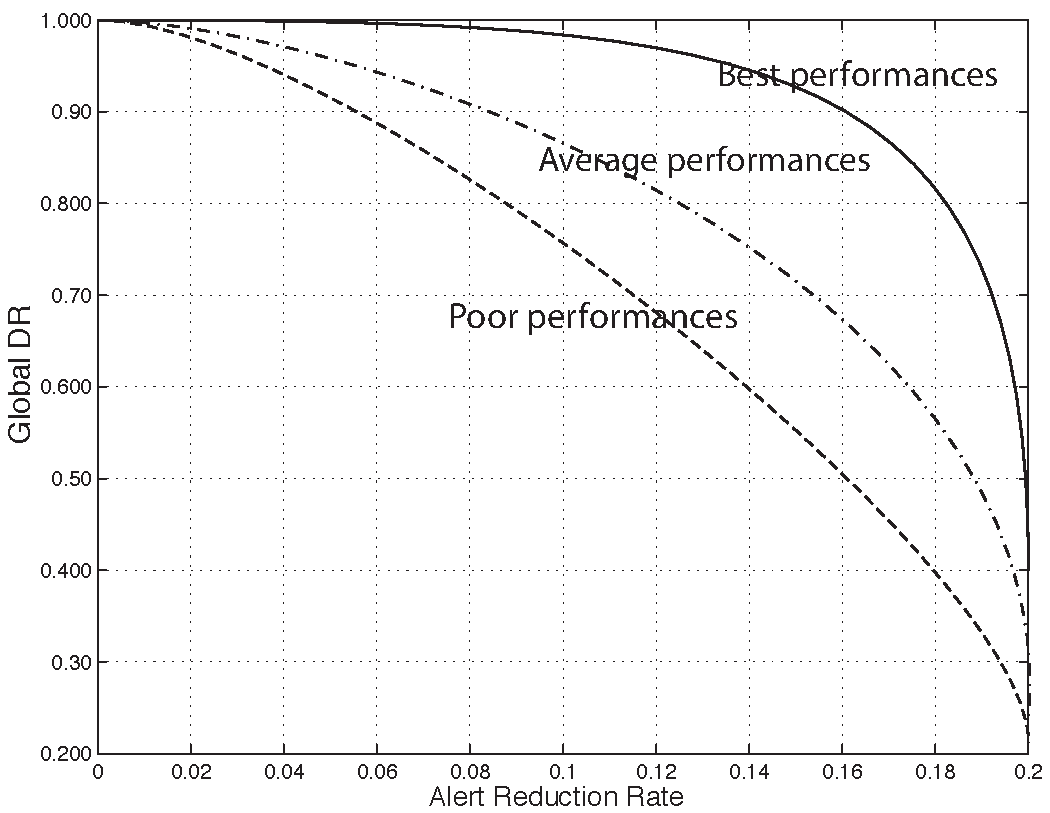
\includegraphics[width=0.8\textwidth]{figures/correlation/evaluation/dummy_dr}\label{subfig:dummy-dr}}
  
  \subfloat[][]{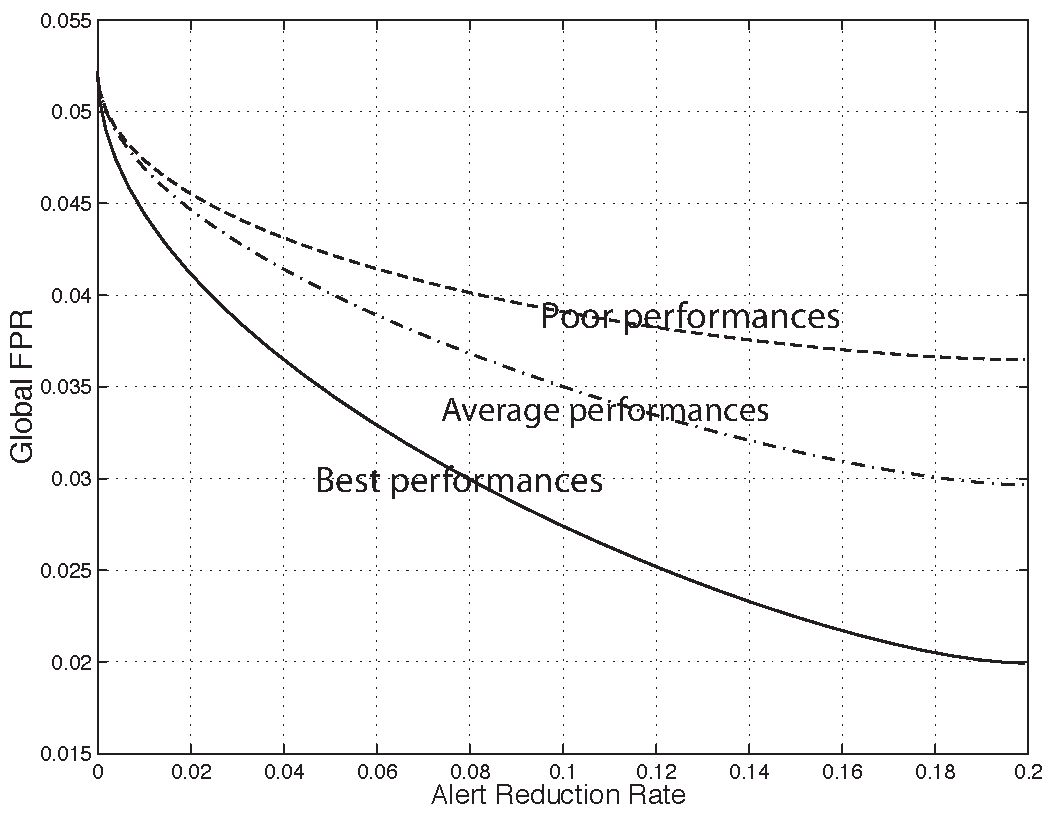
\includegraphics[width=0.8\textwidth]{figures/correlation/evaluation/dummy_fpr}\label{subfig:dummy-fpr}}

  \caption{Hypothetical plots of \subref{subfig:dummy-dr} the global
    DR, $DR_{\mathbb{A}'}$, vs. $ARR$ and \subref{subfig:dummy-fpr}
    the global FPR, $FPR_{\mathbb{A}'}$, vs. $ARR$.}
  \label{fig:dummy}
\end{figure}

Therefore, a fusion system is better than another if it has
\emph{both} a greater $\frac{DR_{\mathbb{A}'}}{DR_{\mathbb{A}}}$ and a
lower $\frac{FPR_{\mathbb{A}'}}{FPR_{\mathbb{A}}}$ rate than the
latter. This criterion by no means has to be considered as complete or
exhaustive. In addition, it is useful to compare $DR_{\mathbb{A}'}$
and $FPR_{\mathbb{A}'}$ plots, vs. $ARR$, of different correlation
systems obtaining diagrams like the one exemplified in Figure
\ref{fig:dummy}; this gives a graphical idea of which correlation
algorithm is better. For instance, Figure \ref{fig:dummy} show that
the algorithm labeled as \textsf{Best performances} is better than the
others, because it shows higher $FPR_{\mathbb{A}'}$ reduction while
$DR_{\mathbb{A}'}$ does not significantly decrease.

\begin{note}[Configuration parameters]
  One limitation of our approach is that it relies on the attack
  belief threshold. Currently, there is no rigorous procedure for
  deriving it in practice. In our experiments, we run the aggregation
  algorithm several times on the same data-set under the same
  conditions until acceptable values of DR and FPR.

  Similarly, the current version of our algorithm relies on alpha cut
  values for deciding whether or not two alerts can be fused or
  not. However, note that this is different from setting thresholds on
  time, e.g., fusing alerts that are delayed, say, 60 seconds. In
  fact, such a threshold would have \emph{direct} impact on the fusion
  procedure; instead, different values of alpha cuts and shapes of
  trapezoid fuzzy sets have a much smoother effects on the results. In
  addition, a user of our system may not be aware of what does it
  means for two alerts to be, say, 60-seconds-close in time; it might
  be easier for the user to just configure the system to fuse alerts
  that are 50\%-close.
\end{note}

\subsection{Experimental Results}
\label{sec:anom-detect-prot}
In these experiments we used two prototypes for network- and
host-based anomaly detection. In particular, we use the system
described in Chapter~\ref{host} (host-based) and
\citep{zanero-savaresi,zanero-pattern} (network-based). These tools
were used to generate alert streams for testing the three variants of
the fuzzy aggregation algorithm we proposed. The same tools were also
used to generate alerts data for testing our correlation algorithm
detailed in Section~\ref{correlation:causality}.

Because of the well known issues of \ac{IDEVAL}\index{IDEVAL} and to
avoid biased interpretation of the results, in our testing we used the
\ac{IDEVAL}\index{IDEVAL} dataset with the following simplification:
we just tried to fuse the stream of alerts coming from a
\ac{HIDS}\index{HIDS} sensor and a \ac{NIDS}\index{NIDS} sensor, which
is monitoring the whole network. To this end, we ran the two
prototypes on the whole 1999 \ac{IDEVAL}\index{IDEVAL} testing
dataset, using the network dumps and the host-based logs from
\texttt{pascal}. We ran the \ac{NIDS}\index{NIDS} prototype on
\texttt{tcpdump} data and collected 128 alerts for attacks against the
host \texttt{pascal.\-eyrie.\-af.\-mil}. The \ac{NIDS}\index{NIDS}
also generated 1009 alerts related to other hosts. Using the
\ac{HIDS}\index{HIDS} prototype we generated 1070 alerts from the
dumps of the host \texttt{pascal.\-eyrie.\-af.\-mil}. The
\ac{NIDS}\index{NIDS} was capable of detecting almost 66\% of the
attacks with less than 0.03\% of false positives; the
\ac{HIDS}\index{HIDS} performs even better with a \ac{DR} of 98\% and
1.7\% of false positives. However, in this experiment we focus on the
aggregated results rather than the detection capabilities of the
single system.

In the following, we use this shorthand notation: $Net$ is the
substream of all the alerts generated by the
\ac{NIDS}\index{NIDS}. $HostP$ is the substream of all the alerts
generated by the \ac{HIDS}\index{HIDS} installed on
\texttt{pascal.\-eyrie.\-af.\-mil}, while $NetP$ regards all the
alerts (with \texttt{pascal} as a target) generated by the
\ac{NIDS}\index{NIDS}; finally, $NetO = Net \backslash NetP$ indicates
all the alerts (with all but \texttt{pascal} as a target) generated by
the \ac{NIDS}\index{NIDS}.

Using the data generated as described above, and the metrics proposed
in Section~\ref{correlation:evaluation:framework}, we compared three
different versions of the alert aggregation algorithms described in
Section \ref{correlation:fusion}. In particular we compare the use of
crisp time-distance aggregation, the use use of a simple fuzzy
time-distance aggregation; and finally, the use of
\texttt{attack\_belief} for alert pruning.

Numerical results are plotted in in Figure \ref{fig:dr_fpr} for
different values of $ARR$. As we discussed in
Section~\ref{correlation:evaluation}, Figure \ref{fig:dr_fpr} (a)
refers to the reduction of \ac{DR} while Figure \ref{fig:dr_fpr} (b)
focuses on \ac{FPR}. $DR_{\mathbb{A}'}$ and $FPR_{\mathbb{A}'}$ were
calculated using the complete alert stream, network and host, at
different values of $ARR$. The values of $ARR$ are obtained by
changing the parameters values: in particular, we set $T_{bel}=0.66$,
the alpha cut of $T_{near}$ to $0.5$, the window size to $1.0$
seconds, and varied the smoothing of the trapezoid between $1.0$ and
$1.5$ seconds, and the alert delay between $0$ and $1.5$ seconds. It
is not useful to plot the increase in false negatives, as it can be
easily deduced from the decrease in \ac{DR}\index{DR}.

\begin{figure}[p]
  \centering
  
  \subfloat[][]{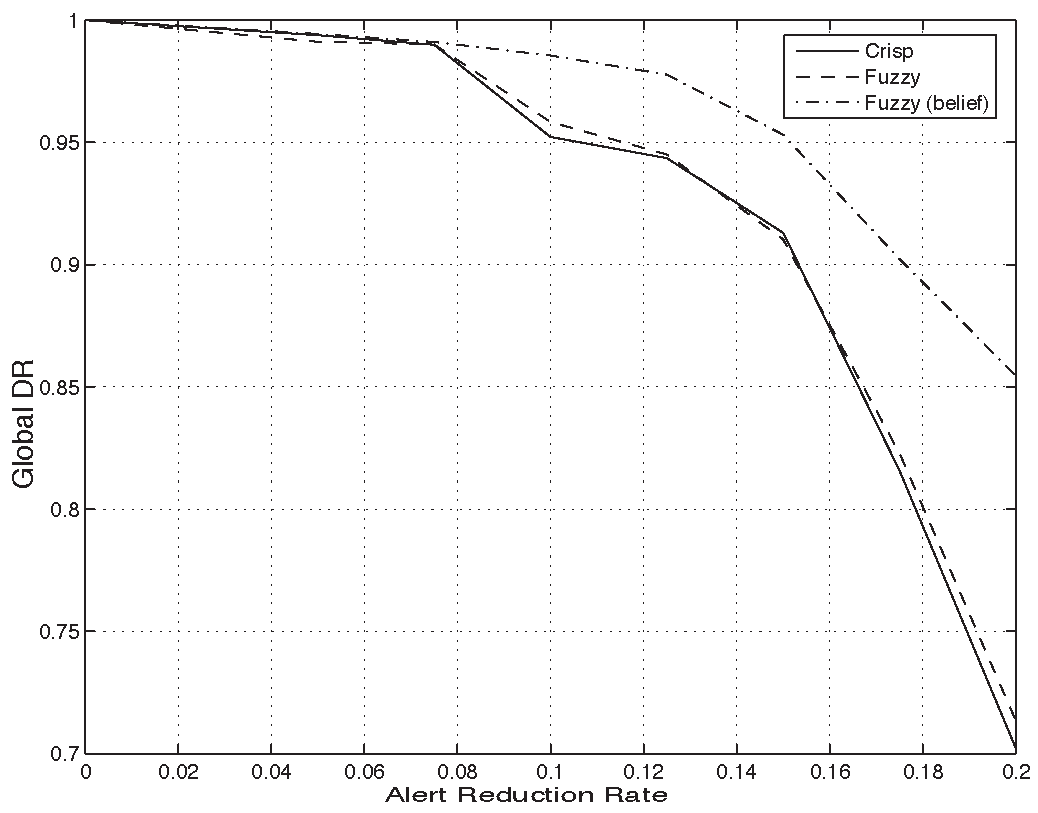
\includegraphics[width=0.8\textwidth]{figures/correlation/fusion/dr_ccf}}
  
  \subfloat[][]{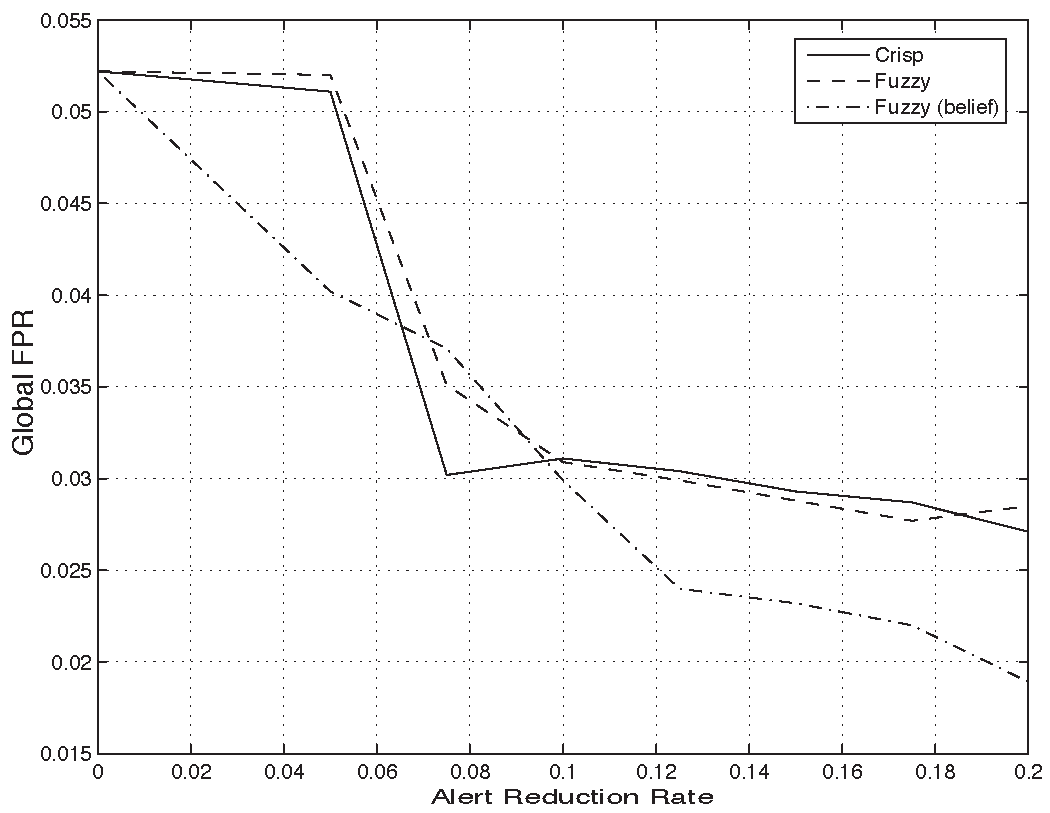
\includegraphics[width=0.8\textwidth]{figures/correlation/fusion/fpr_ccf}}
  
  \caption{Plot of the $DR_{\mathbb{A}'}$ (a) and $FPR_{\mathbb{A}'}$
    (b) vs. $ARR$. ``Crisp'' refers to the use of the crisp
    time-distance aggregation; ``Fuzzy'' and ``Fuzzy (belief)''
    indicates the simple fuzzy time-distance aggregation and the use
    of the \texttt{attack\_belief} for alert discarding,
    respectively.}
  \label{fig:dr_fpr}
\end{figure}

The last aggregation algorithm, denoted as ``Fuzzy (belief)'', shows better performances since the $DR_{\mathbb{A}'}$ is always higher w.r.t. the other two aggregation strategies; this algorithm also causes a significant reduction of the $FPR_{\mathbb{A}'}$. Note that, taking into account the \texttt{attack\_belief} attribute makes the difference because it avoids true positives to be discarded; on the other hand, \emph{real} false positive are not reported in the output alert stream because of their low belief.

It is difficult to properly compare our approach with other other fusion approaches proposed in the reviewed literature, because the latter were not specifically tested from the aggregation point of view, separately from the correlation one. Since the prototypes used to produce results are not released, we are only able to compare our approach with the \emph{overall} fusion systems presented by others. 

\section{Using Non-parametric Statistical Tests}
\label{correlation:causality}
In this section we analyze the use of different types of statistical
tests for the correlation of anomaly detection alerts. We show that
the technique proposed in \citep{dblp:conf/raid/qinl03} and summarized
in Section~\ref{detection:correlation}, one of the few proposals that
can be extended to the anomaly detection domain, strongly depends on
good choices of a parameter which proves to be both sensitive and
difficult to estimate. Rather than using the \acf{GCT} we propose
alternative approach \citep{MaggiZaneroRAID07} based on a set of
simpler statistical tests. We proved that our criteria work well on a
simplified correlation task, without requiring complex configuration
parameters. More precisely, in \citep{MaggiZaneroRAID07} we explored
the use of \emph{statistical causality tests}, which have been
proposed for the correlation of \ac{IDS}\index{IDS} alerts, and which
could be applied to anomaly based \ac{IDS}\index{IDS} as well. We
redefine the problem in terms of a simpler statistical test, and
experimentally validate it.

\subsection{The Granger Causality Test}
\label{correlation:causality:grang-caus-test}
We tested the sensitivity of the \ac{GCT}\index{GCT} to the choice of
two parameters: the sampling time of the time series that represent
the alerts, $w$, and the time lag $l$, i.e., the order of the
\ac{AR}\index{AR} model being fitted. In \citep{dblp:conf/raid/qinl03}
the sampling time was arbitrarily set to $w = 60s$, while the choice
of $l$ is not documented. However, our experiments show that the
choice of these parameters can strongly influence the results of the
test. As explained in \citep{2009_maggi_zanero_matteucci_fusion},
other values of $l$ lead to awkward results.

We used the same dataset described in Section~\ref{sec:anom-detect-prot}, with the following approach: we tested if $NetP$ has any causal relationship\footnote{In the following we will use the symbol ``$\leadsto$'' to denote ``Granger-causes'' so, for instance, ``A $\leadsto$ B'' has to be read as ``A causes B''; the symbol ``$\cancel{\leadsto}$'' indicates the negated causal relationship, i.e., ``does not Granger-cause''.} with $HostP$; we also tested $HostP$ $\cancel{\leadsto}$ $NetP$. Since only a reduced number of alerts was available and since it was impossible to aggregate alerts along the ``attack name'' attribute (unavailable on anomaly detectors), we preferred to construct only two, large time series: one from $NetP$ (denoted as $NetP(k)$) and one from $HostP$ (denoted as $HostP(k)$). In the experiment reported in \citep{dblp:conf/raid/qinl03} the sampling time, $w$, has been fixed at 60 seconds, although we tested different values from 60 to 3600 seconds. In our simple experiment, the expected result is that $NetP \leadsto HostP$, and that $HostP \not\leadsto NetP$ (the $\leadsto$ indicates ``causality'' while $\not\leadsto$ is its negation).

Since the first experiment ($w = 60$) led us to unexpected results (i.e., using a lag, $l$, of $3$ minutes, both $NetP(k)$ $\cancel{\leadsto}$ $HostP(k)$, and vice versa) we decided to plot the test results (i.e., p-value and \ac{GCI}) vs. both $l$ and $w$. In Figure \ref{fig:minute_a0} (a) $l$ is reported in minutes while the experiment has been performed with $w = 60s$; the dashed line is the $p$-value of the test ``$NetP(k)$ $\leadsto$ $HostP(k)$'', the solid line is opposite one. As one may notice, neither the first nor the second test passed, thus nothing can be concluded: fixing the test significance at $\alpha = 0.20$ is the only way for refusing the null hypothesis (around $l \simeq 2.5$ minutes) to conclude both that $NetP \leadsto HostP$'' and that $HostP \cancel{\leadsto} NetP$; the \ac{GCI}\index{GCI} plotted in Figure \ref{fig:minute_a0} (b) confirms the previous result. However, for other values of $l$ the situation changes leading to opposite results.

Figure \ref{fig:hh_a0} shows the results of the test for $w = 1800$ seconds and $l \in [50, 300]$ minutes. If we suppose a test significance of $\alpha = 0.05$ (dotted line), for $l \simeq 120$ the result is that $HostP \leadsto NetP$ while $NetP \cancel{\leadsto} HostP$, the opposite of the previous one. Moreover, for other values of $l$ the $p$-value leads to different results.

The last experiment results are shown in Figure \ref{fig:h_a0}: for $l
> 230$ minutes, one may conclude that $NetP$ $\leadsto$ $HostP$ and
$HostP$ $\cancel{\leadsto}$ $NetP$; i.e., the expected result, even if
the p-value for the second test is close to $\alpha = 0.05$.

\begin{figure}[p]
  \centering
  
  \subfloat[][]{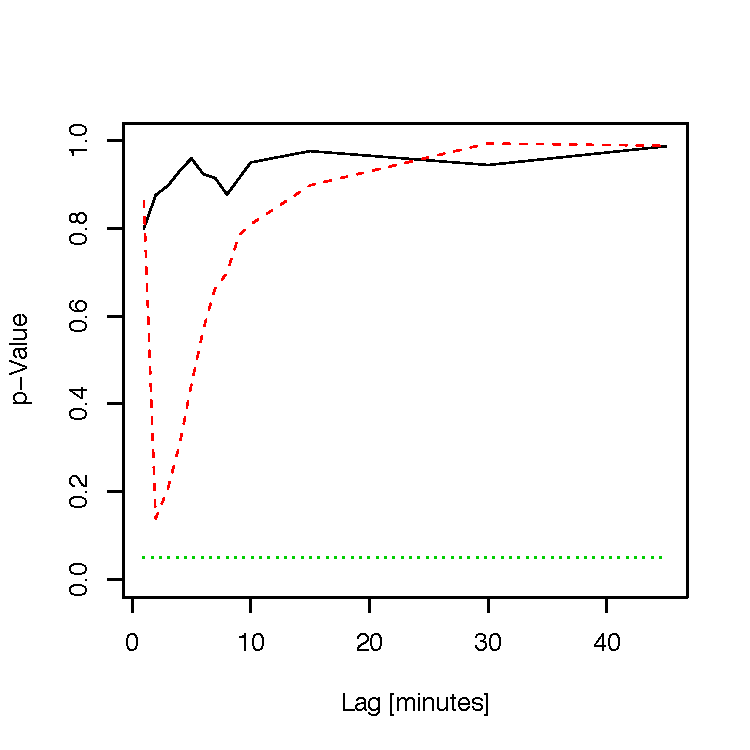
\includegraphics[width=0.8\textwidth]{figures/correlation/fusion/granger/pvalue_minute_a0}}
  
  \subfloat[][]{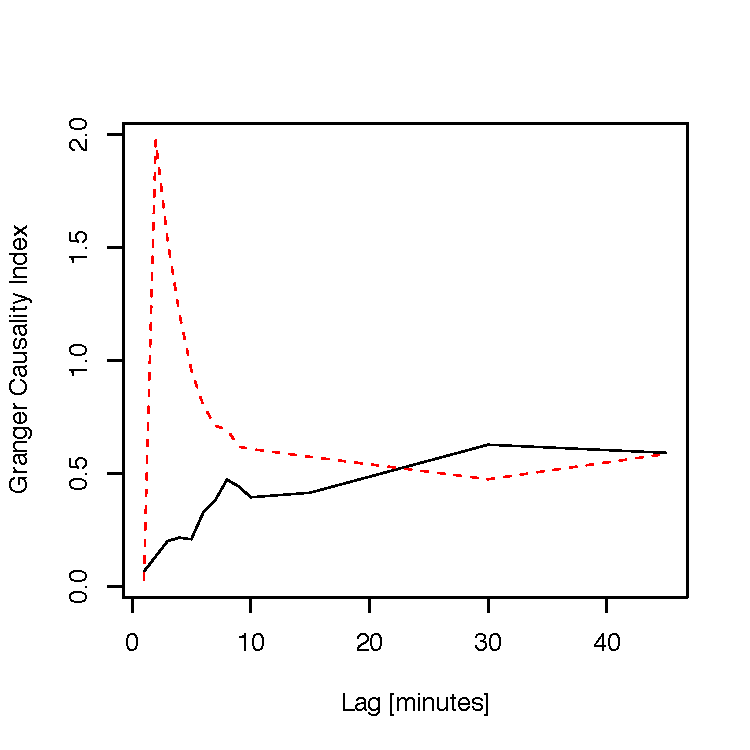
\includegraphics[width=0.8\textwidth]{figures/correlation/fusion/granger/gci_minute_a0}}
  
  \caption{p-value (a) and \ac{GCI} (b) vs. $l$ (in minutes) for the
    first \ac{GCT} experiment ($w = 60.0$ seconds): ``$NetP(k)
    \leadsto HostP(k)$'' (dashed line), ``$HostP(k) \leadsto
    NetP(k)$'' (solid line).}
  \label{fig:minute_a0}
\end{figure}

The previous experiments show only that the \ac{GCT} failed on the dataset we generated, not that it does not work well in general. It may be the case that it is not suitable for ``blind'' alerts (i.e., without any information about the attack) reported by anomaly detectors: in fact, \citep{dblp:conf/raid/qinl03} used time series built from hyper-alerts resulting from an aggregation along \emph{all} attributes: instead, in the anomaly-based case, the lack of attack names does not allow such hyper-alerts to be correctly constructed. In any case, the test result significantly depends on $l$ (i.e., the test is asymptotic); this means that an appropriate choice of $l$ will be required, depending on specific environmental conditions. The optimal $l$ is also likely to change over time in a given environment.

\begin{figure}[p]
  \centering
  
  \subfloat[][]{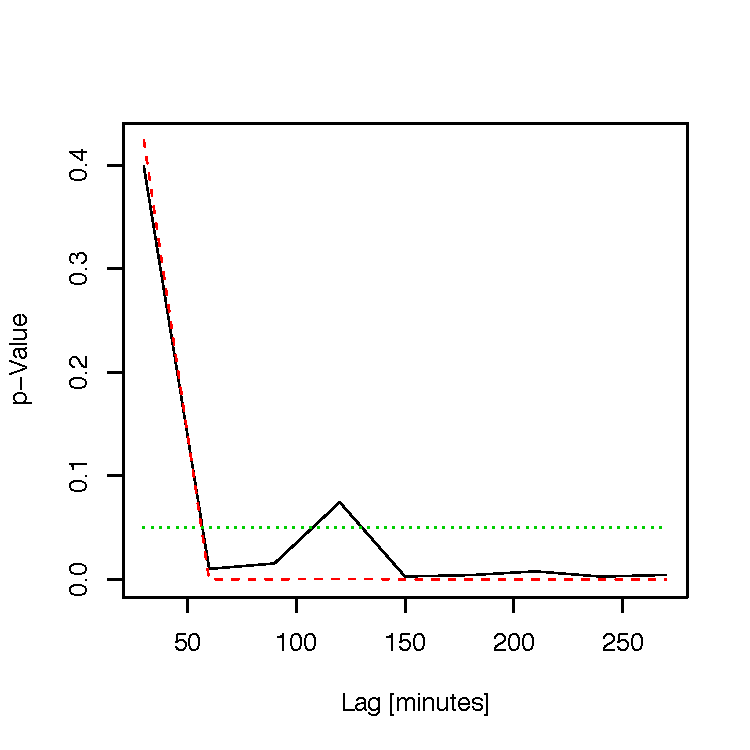
\includegraphics[width=0.8\textwidth]{figures/correlation/fusion/granger/pvalue_hh_a0}}
  
  \subfloat[][]{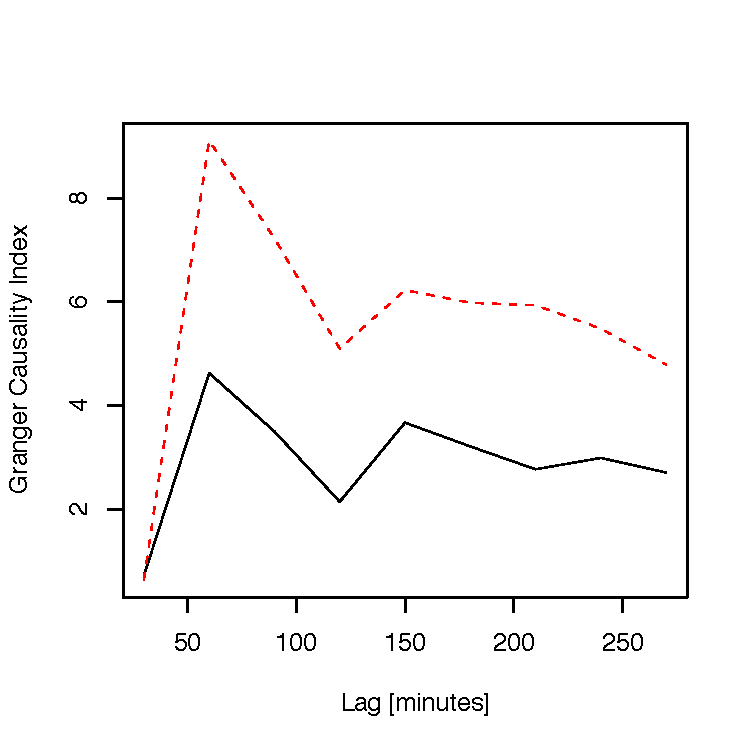
\includegraphics[width=0.8\textwidth]{figures/correlation/fusion/granger/gci_hh_a0}}
  
  \caption{p-value (a) and \ac{GCI}\index{GCI} (b) vs. $l$ (in
    minutes) for the first Granger causality test experiment ($w =
    1800.0$ seconds): ``$NetP(k) \leadsto HostP(k)$'' (dashed line),
    ``$HostP(k) \leadsto NetP(k)$'' (solid line).}
  \label{fig:hh_a0}
\end{figure}

A possible explanation is that the \ac{GCT}\index{GCT} is significant only if both the linear regression models are optimal, in order to calculate the correct residuals. If we use the \ac{AIC} \citep{akaike1974nls} to estimate the optimal time lag $\hat{l}$ over different windows of data, we find out that $\hat{p}$ wildly varies over time, as it is shown in Figure \ref{fig:p-does-vary}. The fact that there is no stable optimal choice of $l$, combined with the fact that the test result significantly depends on it, makes us doubt that the Granger causality test is a viable option for general alert correlation. The choice of $w$ seems equally important and even more difficult to perform, except by guessing.

\begin{figure}[p]
  \centering
  
  \subfloat[][]{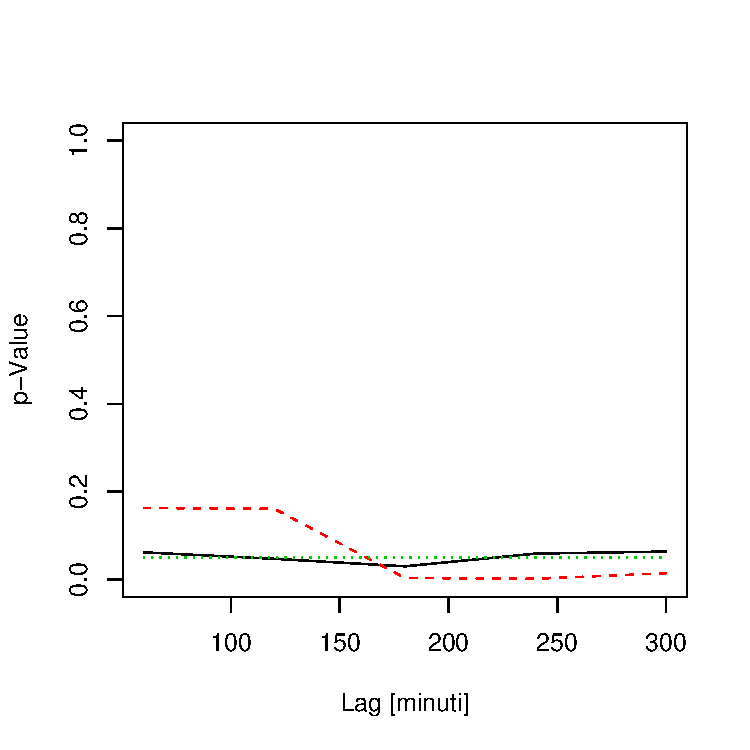
\includegraphics[width=0.8\textwidth]{figures/correlation/fusion/granger/pvalue_h_a0}}
  
  \subfloat[][]{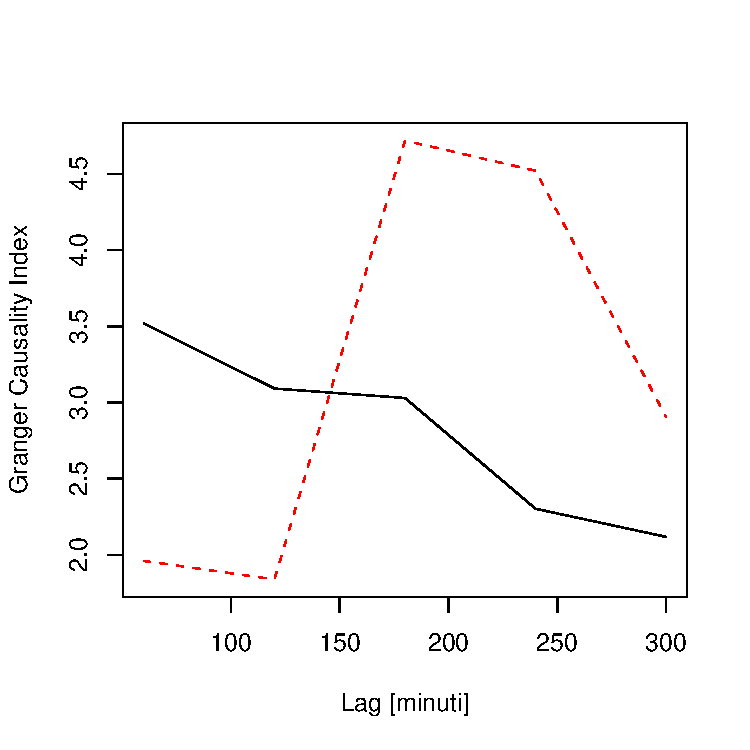
\includegraphics[width=0.8\textwidth]{figures/correlation/fusion/granger/gci_h_a0}}
  
  \caption{p-value (a) and \ac{GCI}\index{GCI} (b) vs. $l$ (in
    minutes) for the first Granger causality test experiment ($w =
    3600.0$ seconds): ``$NetP(k) \leadsto HostP(k)$'' (dashed line),
    ``$HostP(k) \leadsto NetP(k)$'' (solid line).}
  \label{fig:h_a0}
\end{figure}

Of course, our testing is not conclusive: the \ac{IDEVAL}\index{IDEVAL} alert sets may simply not be adequate for showing causal relationships. Another, albeit more unlikely, explanation, is that the \ac{GCT} test may not be suitable for anomaly detection alerts: in fact, in \citep{dblp:conf/raid/qinl03} it has been tested on misuse alerts. But in fact there are also theoretical reasons to doubt that the application of the Granger test can lead to stable, good results. First, the test is asymptotic w.r.t. $l$ meaning that the results reliability decreases as $l$ increases because of the loss of degrees of freedom. Second, it is based on the strong assumption of \emph{linearity} in the auto-regressive model fitting step, which strongly depends on the observed phenomenon. In the same way, the stationarity assumption of the model does not always hold.

\subsection{Modeling alerts as stochastic processes}
\label{correlation:causality:count-proc-model}
Instead of interpreting alert streams as time series (as proposed by
the \ac{GCT}\index{GCT}-based approach), we propose to change point of
view by using a stochastic model in which alerts are modeled as
(random) events in time. This proposal can be seen as a formalized
extension of the approach introduced in \citep{valeur04comprehensive}
(see Figure~\ref{fig:correlation_model}), which correlates alerts if
they are fired by different \ac{IDS}\index{IDS} within a
``negligible'' time frame, where ``negligible'' is defined with a
crisp, fixed threshold.

For simplicity, once again we describe our technique in the simple case of a single \ac{HIDS}\index{HIDS} and a single \ac{NIDS}\index{NIDS} which monitors the whole network. The concepts, however, can be easily generalized to take into account more than two alert streams, by evaluating them couple by couple. For each alert, we have three essential information: a timestamp, a ``target'' host (fixed, in the case of the \ac{HIDS}\index{HIDS}, to the host itself), and the generating sensor (in our case, a binary value).

With a self-explaining notation, define the following random variables: $T_{NetP}$ are the arrival times of network alerts in $NetP$ ($T_{NetO}$, $T_{HostP}$ are similarly defined); $\varepsilon_{NetP}$ ($\varepsilon_{NetO}$) are the delays (caused by transmission, processing and different granularity in detection) between a specific network-based alert regarding \texttt{pascal} (not \texttt{pascal}) and the corresponding host-based one. The actual values of each $T_{(\cdot)}$ is nothing but the set of timestamps extracted from the corresponding alert stream. We reasonably assume that $\varepsilon_{NetP}$ and $T_{NetP}$ are stochastically independent (the same is assumed for $\varepsilon_{NetO}$ and $T_{NetO}$). Figure~\ref{fig:epsilon} shows how delays between network and host alerts are calculated.

\begin{figure}[t]
  \centering
  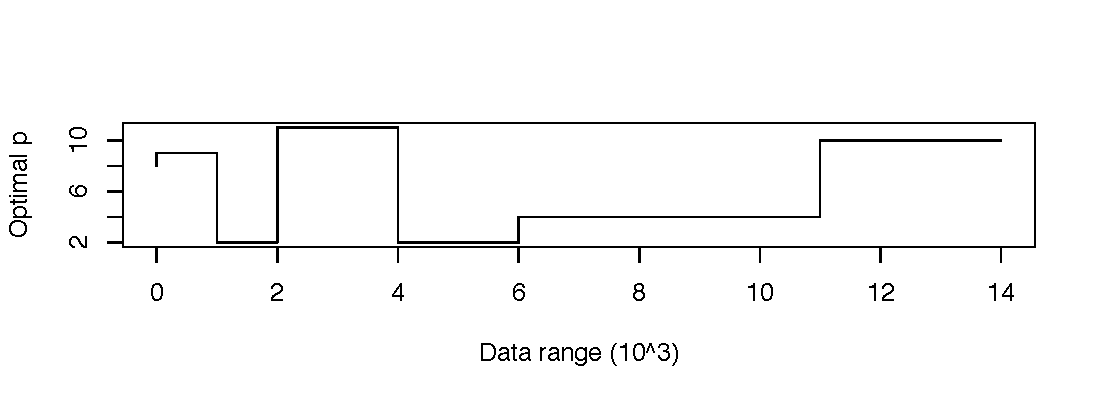
\includegraphics[width=\textwidth]{figures/correlation/causality/p-does-vary}
  \caption{The optimal time lag $p = \hat{l}$ given by the \ac{AIC}
    criterion strongly varies over time.}
  \label{fig:p-does-vary}
\end{figure}

In an \emph{ideal} correlation framework with two equally perfect \ac{IDS}\index{IDS} with a 100\% \ac{DR} and 0\% \ac{FPR}, if two alert streams are correlated (i.e., they represent independent detections of the same attack occurrences by different \acp{IDS}\index{IDS} \citep{valeur04comprehensive}), they also are ``close'' in time. $NetP$ and $HostP$ should evidently be an example of such a couple of streams. Obviously, in the real world, some alerts will be missing (because of false negatives, or simply because some of the attacks are detectable only by a specific type of detector), and the distances between related alerts will therefore have some higher variability. In order to account for this, we can ``cut off'' alerts that are too far away from a corresponding alert in the other time series, presuming them to be singletons. In our case, knowing that single attacks did not last more than $400 s$ in the original dataset, we tentatively set a cutoff threshold at this point.

Under the given working assumptions, the proposed stochastic model is used to formalize the correlation problem as a set of two statistical hypothesis tests:

\begin{equation}\label{eq:hp-test-1}
  \begin{array}{ccc}
    H_{0} && H_{1}\\
    T_{HostP} \neq T_{NetP} + \varepsilon_{NetP} &vs.& T_{HostP} = T_{NetP} + \varepsilon_{NetP}
  \end{array}
\end{equation}

\begin{equation}\label{eq:hp-test-2}
  \begin{array}{ccc}
    T_{HostP} \neq T_{NetO} + \varepsilon_{NetO} &vs.& T_{HostP} = T_{NetO} + \varepsilon_{NetO}
  \end{array}
\end{equation}

Let $\{t_{i,k}\}$ be the observed timestamps of $T_{i}, \forall i \in \{HostP$, $NetP$, $NetO\}$, the meaning of the first test is straightforward: within a random amount of time, $\varepsilon_{NetP}$, the occurring of a host alert, $t_{HostP,k}$, is preceded by a network alert, $t_{NetP,k}$. If this does not happen for a statistically significant amount of events, the test result is that alert stream $T_{NetP}$ is \emph{uncorrelated} to $T_{HostP}$; in this case, we have \emph{enough statistical evidence} for refusing $H_{1}$ and accepting the null one. Symmetrically, refusing the null hypothesis of the second test means that the $NetO$ alert stream (regarding to all hosts but \texttt{pascal}) is correlated to the alert stream regarding \texttt{pascal}.

Note that, the above two tests are strongly related to each other: in an ideal correlation framework, it cannot happen that both ``$NetP$ is correlated to $HostP$'' and ``$NetO$ is correlated to $HostP$'': this would imply that the network activity regarding to all hosts but \texttt{pascal} (which raises $NetO$) has to do with the host activity of \texttt{pascal} (which raises $HostP$) with the same order of magnitude of $NetP$, that is an intuitively contradictory conclusion. Therefore, the second test acts as a sort of ``robustness'' criterion.

\begin{figure}[t]
  \centering
  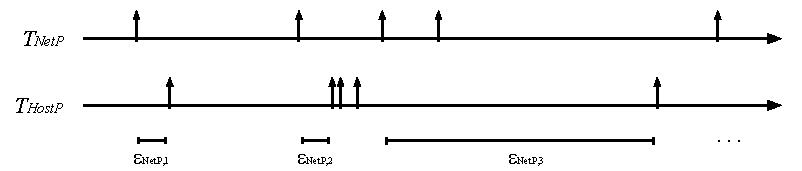
\includegraphics[width=\textwidth]{figures/correlation/causality/epsilon}
  \caption{How delays between network and host alerts are calculated.}
  \label{fig:epsilon}
\end{figure}

From our alerts, we can compute a sample of $\varepsilon_{NetP}$ by simply picking, for each value in $NetP$, the value in $HostP$ which is closest, but greater (applying a threshold as defined above). We can do the same for $\varepsilon_{NetO}$, using the alerts in $NetO$ and $HostP$.

The next step involves the \emph{choice of the distributions} of the random variables we defined above. Typical distributions used for modeling random occurrences of timed events fall into the family of exponential \acp{PDF}\index{PDF} \citep{pestman}. In particular, we decided to fit them with Gamma \acp{PDF}\index{PDF}, because our experiments show that such a distribution is a good choice for both the $\varepsilon_{NetP}$ and $\varepsilon_{NetO}$.

\begin{figure}[t]
  \centering
  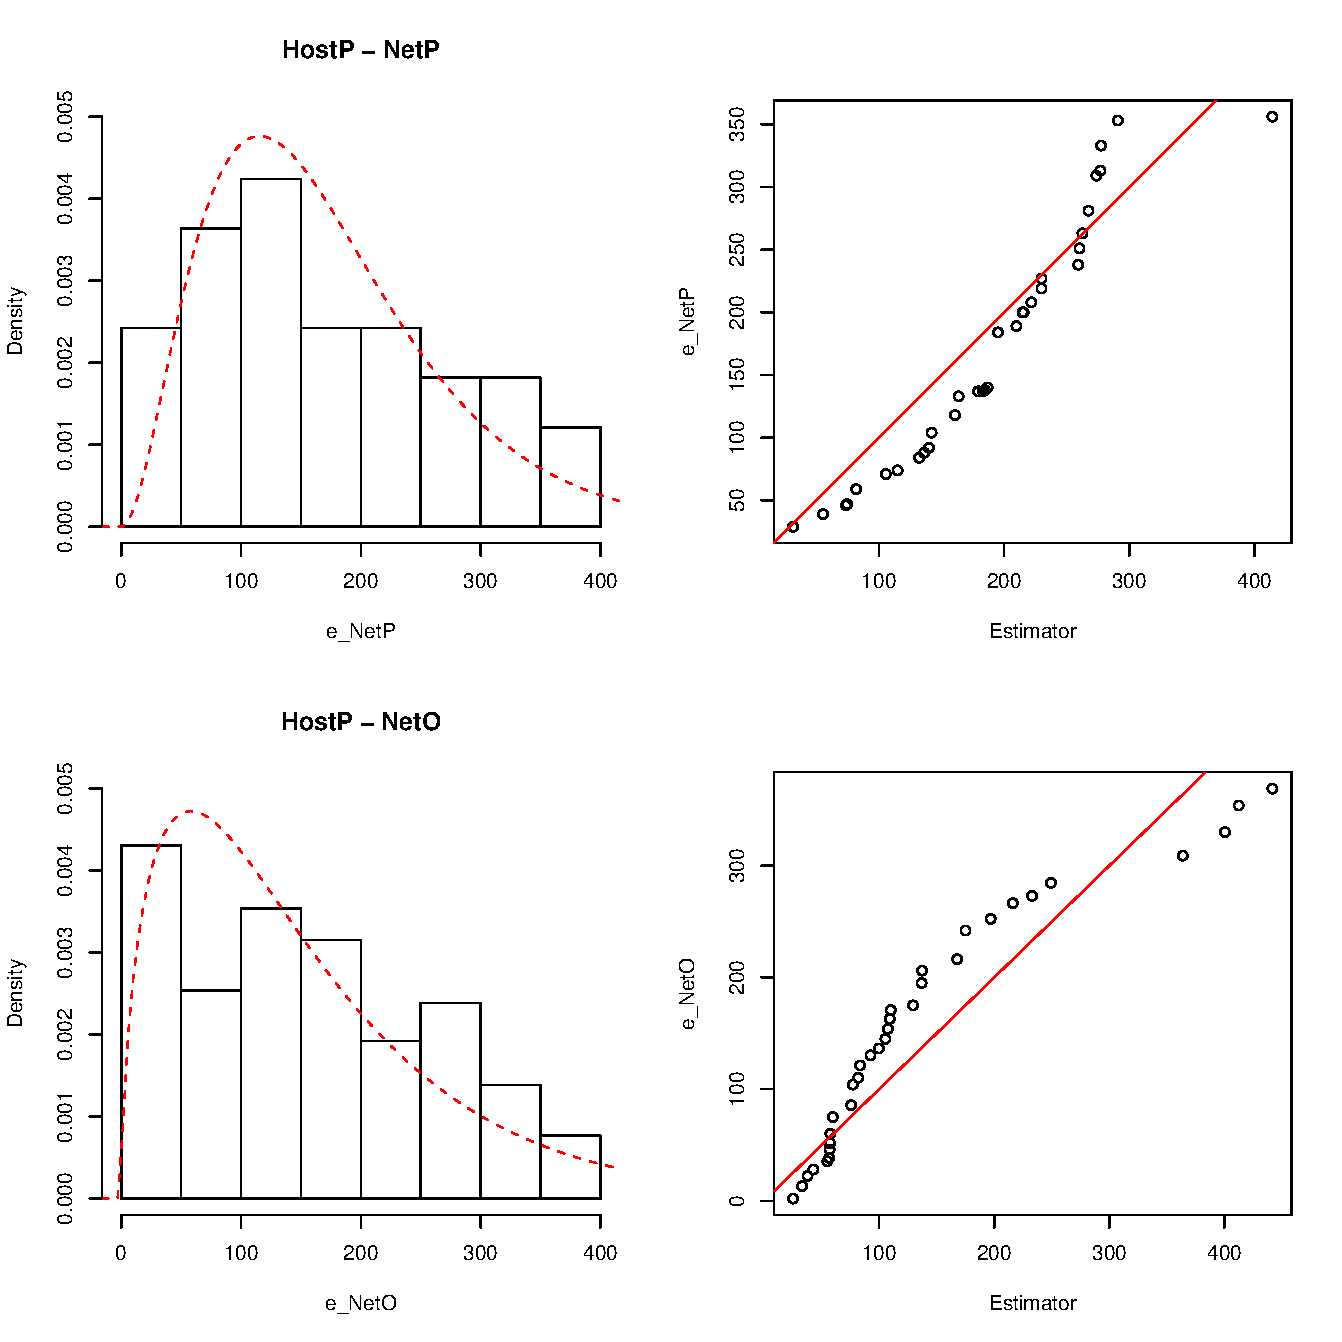
\includegraphics[width=\textwidth]{figures/correlation/causality/hist_qqplot}
  \caption{Histograms vs. estimated density (red dashes) and Q-Q
    plots, for both $\hat{f_{O}}$ and $\hat{f_{P}}$.}
  \label{fig:hist_qqplot}
\end{figure}

The estimation of the \ac{PDF}\index{PDF} of $\varepsilon_{NetP}$,
$f_{P} := f_{\varepsilon_{NetP}}$, and $\varepsilon_{NetO}$, $f_{O} :=
f_{\varepsilon_{NetO}}$, is performed using the well known \ac{ML}
technique \citep{venables2002mas} as implemented in the \textsf{GNU S}
package: the results are summarized in Figure
\ref{fig:hist_qqplot}. $f_{P}$ and $f_{O}$ are approximated by

\begin{displaymath}
  \mathrm{Gamma}(3.0606, 0.0178)
\end{displaymath}

\begin{displaymath}
  \mathrm{Gamma}(1.6301, 0.0105)
\end{displaymath}


\noindent respectively (standard errors on parameters are $0.7080$, $0.0045$ for $f_{P}$ and $0.1288$, $0.009$ for $f_{O}$). From now on, the estimator of a given density $f$ will be indicated as $\hat{f}$.

\begin{figure}[t]
  \centering
  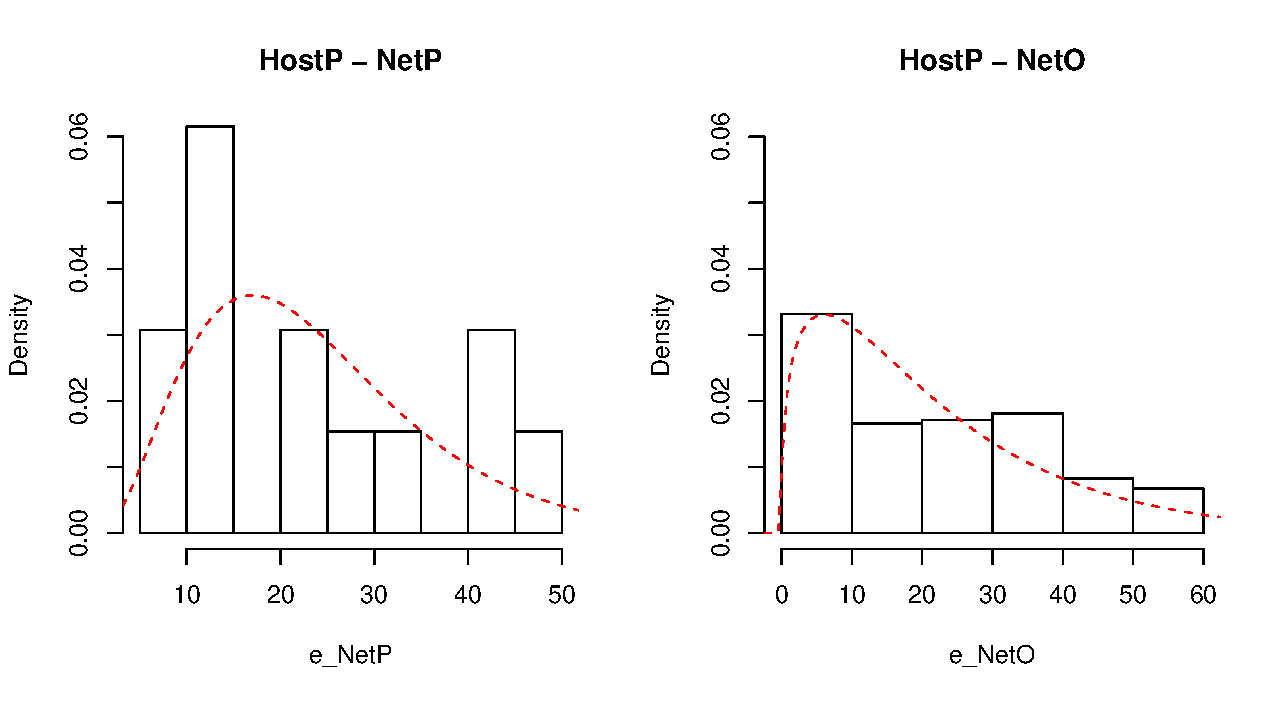
\includegraphics[width=\textwidth]{figures/correlation/causality/hist_1998}
  \caption{Histograms vs. estimated density (red dashes) for
    both $\hat{f_{O}}$ and $\hat{f_{P}}$ (\ac{IDEVAL}\index{IDEVAL} 1998)}
  \label{fig:hist_1998}
\end{figure}

Figure \ref{fig:hist_qqplot} shows histograms vs. estimated density (red, dashed line) and quantile-quantile plots (Q-Q plots), for both $\hat{f}_{O}$ and $\hat{f}_{P}$. We recall that Q-Q plots are an intuitive graphical ``tool'' for comparing data distributions by plotting the quantile of the first distribution against the quantile of the other one.

Considering that the samples sizes of $\varepsilon_{(\cdot)}$ are around 40, Q-Q plots empirically confirms our intuition: in fact, $\hat{f}_{O}$ and $\hat{f}_{P}$ are both able to explain real data well, within inevitable but negligible estimation errors. Even if $\hat{f}_{P}$ and $\hat{f}_{O}$ are both Gamma-shaped, it must be noticed that they significantly differ in their parametrization; this is a very important result since it allows to set up a proper criterion to decide whether or not $\varepsilon_{NetP}$ and $\varepsilon_{NetO}$ are generated by the same phenomenon.

Given the above estimators, a more precise and robust hypotheses test can be now designed. The Test \ref{eq:hp-test-1} and \ref{eq:hp-test-2} can be mapped into two-sided \ac{KS} tests \citep{pestman}, achieving the same result in terms of decisions:

\begin{equation}\label{eq:ks-test-1}
  \begin{array}{ccc}
    H_{0} && H_{1}\\
    \varepsilon_{NetP} \sim f_{P} &vs.& \varepsilon_{NetP} \not\sim f_{P}
  \end{array}
\end{equation}

\begin{equation}\label{eq:ks-test-3}
  \begin{array}{ccc}
    \varepsilon_{NetO} \sim f_{O} &vs.& \varepsilon_{NetO} \not\sim f_{O}
  \end{array}
\end{equation}

where the symbol $\sim$ means ``has the same distribution of''. Since we do not know the real \acp{PDF}\index{PDF}, estimators are used in their stead. We recall that the \ac{KS}\index{KS}-test is a \emph{non-parametric} test to compare a sample (or a \ac{PDF}) against a \ac{PDF} (or a sample) to check how much they differs from each other (or how much they fit). Such tests can be performed, for instance, with \texttt{ks.test()} (a \texttt{GNU R} native procedure): resulting p-values on \ac{IDEVAL}\index{IDEVAL} 1999 are $0.83$ and $0.03$, respectively.

Noticeably, there is a significant statistical evidence to accept the null hypothesis of Test \ref{eq:ks-test-1}. It seems that the \ac{ML}\index{ML} estimation is capable of correctly fitting a Gamma \ac{PDF}\index{PDF} for $f_{P}$ (given $\varepsilon_{NetP}$ samples), which double-checks our intuition about the distribution. The same does not hold for $f_{O}$: in fact, it cannot be correctly estimated, with a Gamma \ac{PDF}\index{PDF}, from $\varepsilon_{NetO}$. The low p-value for Test \ref{eq:ks-test-3} confirms that the distribution of $\varepsilon_{NetO}$ delays is completely different than the one of $\varepsilon_{NetP}$. Therefore, our criterion doest not only recognize noisy delay-based relationships among alerts stream \emph{if they exists}; it is also capable of detecting if such a correlation does not hold.

We also tested our technique on alerts generated by our NIDS and HIDS
running on \ac{IDEVAL}\index{IDEVAL} 1998 (limiting our analysis to
the first four days of the first week), in order to cross-validate the
above results. We prepared and processed the data with the same
procedures we described above for the 1999 dataset. Starting from
almost the same proportion of host/net alerts against either
\texttt{pascal} or other hosts, the \ac{ML}\index{ML}-estimation has
computed the two Gamma densities shown in Figure \ref{fig:hist_1998}:
$f_{P}$ and $f_{O}$ are approximated by $\mathrm{Gamma}(3.5127,
0.1478)$ and $\mathrm{Gamma}(1.3747, 0.0618)$, respectively (standard
errors on estimated parameters are $1.3173$, $0.0596$ for $f_{P}$ and
$0.1265$, $0.0068$ for $f_{O}$). These parameter are very similar to
the ones we estimated for the \ac{IDEVAL}\index{IDEVAL} 1999
dataset. Furthermore, with p-values of 0.51 and 0.09, the two
\ac{KS}\index{KS} tests confirm the same statistical discrepancies we
observed on the 1999 dataset.

\begin{table}[t]
  \centering\footnotesize
  \begin{tabular}{rcccc}
    \toprule
    & \multicolumn{2}{c}{\textsc{IDEVAL 1998}} & \multicolumn{2}{c}{\textsc{IDEVAL 1999}}\\
    \midrule
    & $\alpha$ & $\beta$ & $\alpha$ & $\beta$\\
    \midrule
    $\hat{f_{P}}$ & 3.512 (1.317) & 0.147 (0.059) & 3.060 (0.708) & 0.017 (0.004)\\
    $\hat{f_{O}}$ & 1.374 (0.126) & 0.061 (0.006) & 1.630
    (0.128) & 0.010 (0.009)\\
    \bottomrule
  \end{tabular}
  \caption{Estimated parameters (and their estimation standard error) for the Gamma \acp{PDF}\index{PDF} on \ac{IDEVAL}\index{IDEVAL} 1998 and 1999.}
  \label{tab:1998-1999}
\end{table}

The above numerical results show that, by interpreting alert streams as random processes, there are several (stochastic) dissimilarities between net-to-host delays belonging to the same net-host attack session, and net-to-host delays belonging to different sessions. Exploiting these dissimilarities, we may find out the correlation among streams in an unsupervised manner, without the need to predefine any parameter.

\section{Concluding Remarks}
\label{correlation:conclusions}
In this chapter we first described and evaluated a technique which uses fuzzy sets and measures to fuse alerts reported by the anomaly detectors. After a brief framework description and precise problem statement, we analyzed previous literature about alert fusion (i.e., aggregation and correlation), and found that effective techniques have been proposed, but they are not really suitable for anomaly detection, because they require a-priori knowledge (e.g., attack names or division into classes) to perform well.

Our proposal defines simple, but robust criteria for computing the time distance between alerts in order to take into account uncertainty on both measurements and the threshold-distance sizing. In addition, we considered the implementation of a post-aggregation phase to remove non-aggregated alerts according to their belief, a value indicating how much the \ac{IDS}\index{IDS} believes the detected attack to be real. Moreover, we defined and used some simple metrics for the evaluation of alert fusion systems. In particular, we propose to plot both the \ac{DR} and the \ac{FPR} vs. the degree of output alert reduction vs. the size of the input alert stream.

We performed experiments for validating our proposal. To this end, we used two prototypes we previously developed: a host anomaly detector, that exploits the analysis of system calls arguments and behavior, and a network anomaly detector, based on unsupervised payload clustering and classification techniques that enables an effective outlier detection algorithm to flag anomalies. During our experiments, we were able to outline many shortcomings of the \ac{IDEVAL}\index{IDEVAL} dataset (the only available \ac{IDS}\index{IDS} benchmark) when used for evaluating alert fusion systems. In addition to known anomalies in network and host data, \ac{IDEVAL}\index{IDEVAL} is outdated both in terms of background traffic and attack scenarios.

Our experiments showed that the proposed fuzzy aggregation approach is able to decrease the \ac{FPR} at the price of a small reduction of the \ac{DR} (a necessary consequence). The approach defines the notion of ``closeness'' in time as the natural extension of the naive, crisp way; to this end, we rely both on fuzzy set theory and fuzzy measures to semantically ground the concept of ``closeness''. By definition, our method is robust because it takes into account major uncertainties on timestamps; this means the choice of window size is less sensitive to fluctuations in the network delays because of the smoothing allowed by the fuzziness of the window itself. Of course, if the delays are varying too much, a dynamic resizing is still necessary. The biggest challenge with our approach would be its extension to the correlation of distributed alerts: in the current state, our modeling is not complete, but can potentially be extended in such a way; being the lack of alert features the main difficult.

Secondly, we analyzed the use of of different types of statistical tests for the correlation of anomaly detection alerts, a problem which has little or no solutions available today. One of the few correlation proposals that can be applied to anomaly detection is the use of a \ac{GCT}. After discussing a possible testing methodology, we observed that the \ac{IDEVAL}\index{IDEVAL} datasets traditionally used for evaluation have various shortcomings, that we partially addressed by using the data for a simpler scenario of correlation, investigating only the link between a stream of host-based alerts for a specific host, and the corresponding stream of alerts from a network based detector.

We examined the usage of a \ac{GCT}\index{GCT} as proposed in earlier works, showing that it relies on the choice of non-obvious configuration parameters which significantly affect the final result. We also showed that one of these parameters (the order of the models) is absolutely critical, but cannot be uniquely estimated for a given system. Instead of the \ac{GCT}\index{GCT}, we proposed a simpler statistical model of alert generation, describing alert streams and timestamps as stochastic variables, and showed that statistical tests can be used to create a reasonable criterion for distinguishing correlated and non correlated streams. We proved that our criteria work well on the simplified correlation task we used for testing, without requiring complex configuration parameters.

These were exploratory works, and further investigations on longer
sequences of data, as well as further refinements of the tests and the
criteria we proposed, are surely needed. Another possible extension of
this work is the investigation of how these criteria can be used to
correlate anomaly and misuse-based alerts together, in order to bridge
the gap between the existing paradigms of intrusion detection. In
particular, another possible correlation criteria could be build upon
the observation that a compromised host behaves differently (e.g., its
response time increases).

%%% Local Variables: 
%%% mode: latex
%%% TeX-master: "thesis"
%%% End: 
